\section{Preliminaries}
\label{sec:preliminaries}

Let $\integerball{b} \defeq (-b,b) \cap \integers$ and $[a] \defeq [1,a] \cap \integers$. For a ring $\ring$ of degree $\ringdegree$, let $\vec{r} \in \integers^\ringdegree$ denote the coefficient vector of $r \in \ring$ in the integral basis.

For $m \in \naturals$, let $\zeta_m \in \cmplx$ be any fixed primitive $m$-th root of unity.  Let $\ring = \integers[\zeta_m]$ denote its ring of integers, called a cyclotomic ring.  We have $\ring \cong \integers[x]/\langle \Phi_m(x) \rangle$, where $\Phi_m(x)$ is the $m$-th cyclotomic polynomial.  If $m$ is a power of 2, we call $\ring$ a power-of-2 cyclotomic ring.  In this paper, we exclusively use power-of-2 cylotomic rings.  Let $\modulus \in \naturals$ be a prime number, we let $\fring \defeq \ring/\modulus\ring$ and let $\fring^\times$ denote all invertible elements in $\fring$.
For any $f \in \ring$, let $\mathsf{ct}(f)$ denote the constant term of $f$ (i.e., $\mathsf{ct}(f) = \vec{f}_0$).

For $x \in \ring$, let $\norm{x}$ denote the $\ell$-infinity norm of its coefficient vector, i.e., $\norm{x} = \max_{i \in [\ringdegree]} \vec{x}$.  We use $\norm{\cdot}_p$ for the $\ell_p$-norm (e.g., $\norm{\cdot}_2$ for the $\ell_2$ norm).

\begin{definition}[Ring expansion factor] \label{def:ring-expansion-factor}
Let $\ring$ be a ring.  The \emph{expansion factor} of $\ring$ is defined as $\expansionfactor := \max_{a, b \in \ring} \frac{\norm{a \cdot
b}}{\norm{a}\cdot\norm{b}}$.
\end{definition}

\begin{theorem}[\cite{C:AlbLai21}] \label{thm:expansion-factor}
        If $\ring = \integers[\zeta_m]$ is a power-of-2 cyclotomic ring, then $\expansionfactor \leq \ringdegree$.
\end{theorem}

\begin{theorem}[\cite{C:ACLMT22}] \label{thm:invertibility}
        Let $q = \omega((w\cdot f)^{f/\phi(m)})$ be a rational prime such that $\fring$ splits into $f$ fields each of size $q^{\phi(m)/f}$. For $\varv \randpick \fring^w$, we have $\varv \in (\fring^\times)^w$ with probability $(1 - 1/q^{\phi(m)/f})^{w\cdot f}$.
\end{theorem}

Subsequently in this work, we set $q$ large enough so that uniformly random $v \randpick \fring$ satisfies $v \in \fring^\times$ with non-negligible probability.

\parhead{The conjugation automorphism}
\label{sec:automorphism}
The cyclotomic ring $\ring$ has a group of automorphisms $\automorphism{\ring}$ that is isomorphic to $\ZZ^\times_{2\ringdegree}$,
\[
i \to \sigma_i : \ZZ^\times_{2\ringdegree} \to \automorphism{\ring}
\]
We make use of the following property: given two vectors $\vec{a} = (a_0, \dots, a_{k\ringdegree - 1}) \in \ZZ^{k\ringdegree}$, $\vec{b} = (b_0, \dots, b_{k\ringdegree - 1}) \in \ZZ^{k\ringdegree}$ where $k \geq 1$   , let $c \gets \sum_{i = 0}^{k - 1} \sigma_{-1}(\sum_{j = 0}^{\ringdegree - 1} a_{i\cdot \ringdegree +j} X^j) \cdot (\sum_{j = 0}^{\ringdegree - 1} b _{i\cdot \ringdegree +j} X^j) \in \ring$; then the constant coefficient denoted as $\mathsf{ct}(c)$ has the property that $\mathsf{ct}(c) = \innerproduct{\vec{a}}{\vec{b}}$ (adapted from \cite[Lemma 2.4]{LNP22}, see also \cite{ENS20}).

%%%%%%%%%%%%%%%%%%%%%%%%%%%%%%%%%%%%%%%%%%%%%%%%%%%%%%%%%%%%%%%%%%%%%%%%%%%%%%%%
%%%%%%%%%%%%%%%%%%%%%%%%%%%%%%%%%%%%%%%%%%%%%%%%%%%%%%%%%%%%%%%%%%%%%%%%%%%%%%%%
\subsection{Exceptional challenge sets}
\label{sec:challenges}

For a cyclotomic ring $\ring$ of degree $n$, let $\challengeset \subset \ring$ be the set of ring elements with $c$ plus or minus one coefficients and $n-c$ zero coefficients. Then $\vert\challengeset\vert = 2^c \binom{n}{c}$, and if $\fring$ is a power-of-two cyclotomic, the operator norm of $\challengeset$ with respect to the $\ell$-infinity norm is $c$, i.e., $\mathsf{op}(\challengeset) = c$ (\cref{lemma:op-norm}). By \cite[Corollary 1.2]{ls20} for $n$ a power of two and $q \equiv 2n+1 \bmod 4n$ prime the $2n$-th cyclotomic polynomial $X^n+1$ splits completely into linear factors modulo $q$.\footnote{A close reading of the proof reveals for the fully splitting case that the simpler condition $q \equiv 1 \bmod n$ suffices.} Further, infinitely many such primes $q$ exist and for any $h \in \ring$ that satisfies $0 < \ltwonorm{h} < q^{1/n}$ has an inverse in $\fring$. We wish to ensure that the difference between any two distinct elements in the challenge set is not a zero divisor, i.e., $\challengeset$ is \emph{exceptional}, in order to invoke the following theorem.

% for deg(f) = d
% N = n|H|-d balls
% min sum_i b_i = n balls prefilled in bins
% distribute the n|H|-(n+d) remaining balls so as to minimize \prod_i y_i
% if d < |H|, then
% min \prod_i y_i = |H|^{n-1} (|H|-d)
% H^t - H^t + H^{t-1} = 1 / |H|
\begin{theorem}[Generalized Alon--F{\"u}redi Theorem~\cite{BCPS18}]
\label{thm:alon-furedi}
Let $\ring$ be a ring and let $\challengeset$ be an exceptional, non-empty, finite subset of \ring. Then for any non-zero polynomial $f \in \ring[Y_1,\ldots,Y_t]$ such that $\deg(f) < |H|$ it holds that
\[
        \Pr[f(h_1,\ldots,h_t) = 0  \ | \ h_1,\dots,h_t \randpick \challengeset] \leq \frac{\deg(f)}{\vert\challengeset\vert}
        \enspace.
\]
\end{theorem}

Concretely, for $\deg(f)=1$ and $c=19$ the right-hand of side of the inequality above is $<2^{-132}$. We know that differences $c_i - c_j$ for $c_i \neq c_j \in \challengeset$ with $19$ $\pm 2$ coefficients can be reduced to the invertibility of $2$ and polynomials with $18$ $\pm 1$ coefficients. Differences with $18$ $\pm 2$ coefficients and $2$ $\pm 1$ coefficients have $\ell_2$ norm $\sqrt{74}$. We must then have $q \geq 2^{1590} > \sqrt{74}^{512}$. It turns out even larger $q$ are optimal for proof size for concrete instantiations of our scheme capable of handling large circuits.

\begin{lemma}[Operator norm of sparse ternary sets]
        \label{lemma:op-norm}
        For power-of-two $n$, let $\ring = \integers[X]/(X^{n}+1)$ and $1 \leq c \leq n$. The set
        \[
                \challengeset = \set{h \in \fring \pST \|h\|_{\infty} = 1 \And \|h\|_1 = c}.
        \]
        \noindent has operator norm
        \[
                \textsf{op}_{\infty}(\challengeset) = \max_{h \in \challengeset, r \in \ring} \frac{\linfinitynorm{hr}}{\linfinitynorm{h}\linfinitynorm{r}} = c
        \]
\end{lemma}
\begin{proof}
Let $\symbfup{r},\symbfup{c}$ be the coefficients of $r$ and $c$. Let $g = rc$ with coefficient vector $\symbfup{g}$. Then
\[
g_k = \sum_{i+j = k} r_i c_j - \sum_{i+j = n + k} r_i c_j
\]
Fixing any $j,k \in \set{0,\dotsc,n-1}$, there is exactly one $i \in \set{0,\dotsc,n-1}$ such that either $i+j = n$ or $i+j = n + k$. Therefore, each coefficient $g_k$ can be bounded by $c \linfinitynorm{r}$.
\end{proof}

%%%%%%%%%%%%%%%%%%%%%%%%%%%%%%%%%%%%%%%%%%%%%%%%%%%%%%%%%%%%%%%%%%%%%%%%%%%%%%%%
%%%%%%%%%%%%%%%%%%%%%%%%%%%%%%%%%%%%%%%%%%%%%%%%%%%%%%%%%%%%%%%%%%%%%%%%%%%%%%%%
\subsection{Functional commitments}
\label{sec:functional-commitments}

\begin{definition}[Functional commitment] \label{def:functional-commitment}
        A (pre-processing non-interactive) functional commitment (FC) scheme is parameterized by a function family
        \[
        \begin{array}{rl}
                % \functionfamily &\defeq \set{\functionfamily_{\publicinputdim,\secretinputdim,\numoutputs} \subseteq \set{\function: \ring^\publicinputdim \times \ring^\secretinputdim \to \ring^\numoutputs}}_{\publicinputdim,\secretinputdim,\numoutputs \in \naturals} \\
                % \functionfamily &\defeq \set{\functionfamily_{\publicinputdim,\secretinputdim} \subseteq \set{\function: \ring^\publicinputdim \times \ring^\secretinputdim \to \ring}}_{\publicinputdim,\secretinputdim \in \naturals} \\
                \functionfamily &\defeq \set{\functionfamily_{\secretinputdim} \subseteq \set{\function: \inputalphabet^\secretinputdim \to \imagespace}}_{\secretinputdim \in \naturals} \\
                % \outputfunctionfamily &\defeq \set{\outputfunctionfamily_{\publicinputdim,\numoutputs} \subseteq \set{\function: \ring^\publicinputdim \to \ring^\numoutputs}}_{\publicinputdim,\numoutputs \in \naturals}
        \end{array}
        \]
        over a ring $\ring$ for input alphabet $\inputalphabet \subseteq \ring$ and image space $\imagespace \subseteq \ring$,
        % where $\publicinputdim,\secretinputdim,\numoutputs$ are the dimensions of the public input, secret input, and output, respectively.
        % where \publicinputdim and \secretinputdim are the dimensions of the public input and secret input, respectively.
        where \secretinputdim is the dimension of the secret (committed) input.
        The FC scheme is defined by a $5$-tuple of PPT algorithms \functionalcommitmentalgs, working as follows:
        \begin{itemize}[nosep]
                % \item $\setup(1^\secparam,1^\publicinputdim,1^\secretinputdim) \to \commitmentkey$: Given (in unary) security parameter \secparam, public input dimension \publicinputdim, and secret input dimension \secretinputdim, samples commitment key \commitmentkey.
                \item $\setup(1^\secparam,1^\secretinputdim) \to (\commitmentkey,\vk)$: Input (in unary) security parameter \secparam and secret input dimension \secretinputdim, samples commitment key \commitmentkey and verification key $\vk$.
                \item $\commit(\commitmentkey,\secretinputvector) \to (\commitment,\proofknowledge)$: Input commitment key \commitmentkey and secret input $\secretinputvector \in \inputalphabet^\secretinputdim$, computes commitment \commitment and a proof of knowledge \proofknowledge of vector \secretinputvector such that $\commitment = \commit(\commitmentkey, \secretinputvector)$.
                % \item $\open(\commitmentkey, \function, \publicinput, \secretinputvector) \to \proofopening$: Input commitment key \commitmentkey, function $\function \in \functionfamily_{\publicinputdim,\secretinputdim}$, public input $\publicinput \in \ring^\publicinputdim$, and secret input $\secretinputvector \in \ring^\secretinputdim$ computes opening proof $\proofopening$ for the evaluation $\function(\publicinput,\secretinputvector)$.
                \item $\open(\commitmentkey, \function, \secretinputvector) \to \proofopening$: Input commitment key \commitmentkey, function $\function \in \functionfamily_{\secretinputdim}$, and secret input $\secretinputvector \in \ring^\secretinputdim$, computes opening proof $\proofopening$ for the evaluation $\function(\secretinputvector)$.
                % \item $\preverify(\commitmentkey, \function) \to \vkf$: Input commitment key \commitmentkey and function $\function \in \functionfamily_{\publicinputdim,\secretinputdim}$, computes preprocessed commitment key \vkf. Preprocessing is done just once per function and allows \verify to run in time sublinear in \function.
                \item $\preverify(\commitmentkey, \function) \to \vkf$: Input verification key $\vk$ and function $\function \in \functionfamily_{\secretinputdim}$, computes preprocessed commitment key $\vkf$. Preprocessing only needs to be performed once per function and allows $\verify$ to run in time sublinear in $\function$.
                % \item $\verify(\vkf,\commitment,\publicinput,\output,\proofopening)$: Input preprocessed commitment key \vkf, commitment \commitment, public input $\publicinput \in \ring^\publicinputdim$, output $\output \in \ring$, and proof \proofopening, return $1$ if the proof is valid (else $0$).
                \item $\verify(\vkf,\commitment,\output,\proofknowledge,\proofopening) \to \bits$: Input preprocessed verification key \vkf, commitment \commitment, output $\output \in \imagespace$, and proofs \proofknowledge and \proofopening, the verifier returns $1$ if the proofs convince them the verifier knows some $\secretinputvector \in \inputalphabet^\secretinputdim$ such that $\commit(\commitmentkey,\secretinputvector) = \commitment$ and $\function(\secretinputvector) = \output$ (else $0$).
        \end{itemize}
\end{definition}

\noindent We require that functional commitments satisfy correctness, extractability, and succinctness as defined below.

\begin{definition}[Correctness] 
\label{def:correctness}
An FC scheme for $(\functionfamily, \inputalphabet,\imagespace)$ is \emph{correct} if for any $\secparam, \secretinputdim \in \naturals$, any $\commitmentkey \gets \setup(1^\lambda, 1^\secretinputdim)$, and for any $(\function, \secretinputvector, \output) \in \functionfamily \times \inputalphabet^\secretinputdim \times \imagespace$ satisfying $\function(\secretinputvector) = \output$, any $(\commitment,\proofknowledge) \gets \commit(\commitmentkey, \secretinputvector)$, any $\proofopening \gets \open(\commitmentkey, \function,\secretinputvector)$, and any $\vkf \gets \preverify(\commitmentkey, \function)$, it holds that $\Pr[\verify(\vkf, \commitment, \output, \proofknowledge, \proofopening) = 1] = 1$.
\end{definition}

At a high level, extractability of an FC scheme requires that if an adversary
can produce a commitment $\commitment$ and a valid opening $(\proofknowledge,\proofopening)$ for some function $\function$ and some evaluation $\output$, it must know $\secretinputvector \in \inputalphabet^\secretinputdim$ satisfying $\commit(\commitmentkey,\secretinputvector) = \commitment$ and $\function(\secretinputvector) = \output$.  Note that extractability implies \emph{weak binding} (meaning that it is not possible to open a commitment to two different evaluations for the same function).

\begin{definition}[Extractability]
\label{def:extractability-fc}
A FC scheme for $(\functionfamily, \inputalphabet,\imagespace)$ is $(\kappa, \inputalphabetasterisk)$-\emph{extractable} if for any PPT adversary $\adversary$, there exists a PPT extractor $\extractoradversary$ that, input $(\commitmentkey,\vk)$ and given black-box access to \adversary and any randomness it uses, returns $\secretinputvectorextracted \in (\inputalphabetextracted)^\secretinputdim$ such that
\begin{equation*}
\mathrm{Pr}\left[
\begin{array}{ll|r}
& \verify(\vkf,\commitment,\output,\proofknowledge,\proofopening) = 1
& (\commitmentkey,\vk) \gets \setup(1^\secparam,1^\secretinputdim) \\
\And& \left(
\begin{array}{ll}
& \secretinputvector \notin (\inputalphabetasterisk)^\secretinputdim \\
\Or& \commitment \neq \commit(\commitmentkey, \secretinputvector, )\\
\Or& \function(\secretinputvector) \neq \output
\end{array}
\right)
& \begin{array}{r}
(\function, \commitment, \output, \proofknowledge,\proofopening) \gets \adversary(\commitmentkey, \vk) \\
\secretinputvector \gets \extractoradversary(\commitmentkey, \vk) \\
\vkf \gets \preverify(\vk, \function)
\end{array}
\end{array}
\right]
\leq \kappa(\secparam,\secretinputdim)
\enspace.
\end{equation*}
We say the scheme is $\inputalphabetasterisk$-extractable if its \emph{knowledge error} $\knowledgeerror(\secparam,\secretinputdim)$ is negligible in $\secparam$ for $\secretinputdim = \poly(\secparam)$.
\end{definition}

\begin{definition}[Succinctness] \label{def:succinctness}
        Let $\Pi$ be a VC scheme for the alphabet $\inputalphabet = \set{r \in \ring \pST \norm{r} \leq \alpha}$. We say $\Pi$ is \emph{succinct} if it satisfies the following properties:
        \begin{itemize}[nosep]
        \item \emph{Proof succinctness}: $\vert \commitment + \proofknowledge + \proofopening \vert = \poly(\log\secretinputdim + \log\normboundinput)$.
        \item \emph{Verifier succinctness}: $\verify$ runs in time $\poly(\log\secretinputdim + \log\normboundinput)$.
        \end{itemize}
\end{definition}

% Collapse-binding was first defined in \cite{unruh16}. We use an equivalent, but more simply stated formulation from~\cite{ds22}.

% \begin{definition}[Collapse-binding] \label{def:collapse-binding}
%         For an adversary \adversary define the experiment $\collapseexperiment$ as follows:
%         \begin{enumerate}[nosep]
%                 \item The challenger generates $\commitmentkey \gets \setup(1^{\secparam})$.
%                 \item $\adversary(\commitmentkey)$ sends a commitment \commitment and the registers \messageregister \tensor \ancillaregister of a quantum state $\rho$.
%                 \item The challenger flips a coin $b \in \set{0,1}$. If $b = 0$, the challenger does nothing. Otherwise, the challenger measures \messageregister in the computational basis.
%                 \item The challenger returns registers \messageregister \tensor \ancillaregister to the adversary, who outputs a bit $b'$. The experiment outputs $1$ if $b = b'$.
%         \end{enumerate}
%         We say \adversary is valid if measuring the output of $\adversary(\commitmentkey)$ in the computational basis yields, with probability $1$, $(\message,\decommitment)$ such that $\commit(\commitmentkey,\message,\decommitment) = \commitment$. We say a commitment scheme is \textsf{collapse-binding} if for all \emph{valid} non-uniform quantum polynomial-time adversaries \adversary
%         \[
%                 \left\vert \prob{\collapseexperiment = 1} - \frac{1}{2} \right\vert = \negl(\secparam)
%                 \enspace.
%         \]
% \end{definition}

%%%%%%%%%%%%%%%%%%%%%%%%%%%%%%%%%%%%%%%%%%%%%%%%%%%%%%%%%%%%%%%%%%%%%%%%%%%%%%%
%%%%%%%%%%%%%%%%%%%%%%%%%%%%%%%%%%%%%%%%%%%%%%%%%%%%%%%%%%%%%%%%%%%%%%%%%%%%%%%
\subsection{Sampling Algorithm}

The following relies on the Leftover Hash Lemma over rings to generate some vector $\publicsisvector$ that is indistinguishable from a uniformly randomly sample vector, and some trapdoor that makes it possible to easily generate vectors in the kernel of $\publicsisvector$.  We let $\lhl(\fring, \normboundpublicpreimages)$ denote an algorithm that outputs the minimum $\ell \in \naturals$, which ensures that the resulting distribution of the vector $\publicsisvector$ is indistinguishable from the uniform distribution. It is formally defined as follows, adapted from \cite{GPV08,EC:MicPei12,GM18,C:ACLMT22}:

A sampling algorithm has the following three PPT algorithms (taking $1^\lambda$ as input implicitly):

\begin{itemize}
    \item $(\publicsisvector, \td) \gets \trapdoorgenerator(1^\numcols, q, \ring, \normboundpublicpreimages)$: takes dimension $\ell \in \naturals$, a modulus $\modulus \in \naturals$, a ring $\ring$, and a norm bound $\normboundpublicpreimages \in \reals$, and outputs a vector $\publicsisvector \in \fring^\ell$ and a trapdoor $\td$. For any $n \in \poly(\lambda), \ell \geq \lhl(\fring, \gadgetbase)$ where $\gadgetbase = O(\normboundpublicpreimages)$, the distribution of $\publicsisvector$ is within $\negl(\secparam)$ statistical distance to $U(\fring^\ell)$. 
    \item $\preimage \gets \sampd(1^\ell, \fring, \normboundpublicpreimages)$: for $\ell \geq \lhl(\fring,\normboundpublicpreimages)$, outputs $\preimage$ such that $\norm{\preimage} \leq \normboundpublicpreimages$ and the distribution of $\innerproduct{\publicsisvector}{\preimage} \modq$ is withing $\negl(\secparam)$ statistical distance to $U(\fring)$.
    \item $\preimage \gets \preimagesampler(\td, \varv, \normboundpublicpreimages)$: for $\ell \geq \lhl(\fring,\normboundpublicpreimages)$ and $\varv \in \fring$, outputs $\preimage \in \ring^\ell_\modulus$ satisfying $\norm{\preimage} \leq \normboundpublicpreimages$, $\innerproduct{\publicsisvector}{\preimage} \equiv \varv \modq$, and that distribution of $\preimage$ is within $\negl(\secparam)$ statistical distance the distribution of $\varv' \gets \sampd(1^\lambda, 1^\ell, \fring, \normboundpublicpreimages)$ conditioned on $\innerproduct{\publicsisvector}{\preimage} \equiv \varv' \modq$.
\end{itemize}


%%%%%%%%%%%%%%%%%%%%%%%%%%%%%%%%%%%%%%%%%%%%%%%%%%%%%%%%%%%%%%%%%%%%%%%%%%%%%%%
%%%%%%%%%%%%%%%%%%%%%%%%%%%%%%%%%%%%%%%%%%%%%%%%%%%%%%%%%%%%%%%%%%%%%%%%%%%%%%%
\subsection{Cryptographic assumptions}

The Short Integer Solution (\sis) problem was first introduced in \cite{Ajt96}, which asks to find a short element (of $\ell_2$ norm) in the kernel of a random matrix over the ring $\integers_\modulus$. An inhomogeneous version, \isis, instead asks for a short solution to some linear equation system~\cite{Mic07}. It has been shown that the \sis and \isis problems are equivalent.

We define the ring version of \sis (\rsis) from \cite{Mic07} as follows.
\begin{definition}[\rsis~\cite{Mic07}] \label{def:rsis}
Let $\ring, \modulus, \numcols, \normboundpublicpreimages$ be parameters depending on $\secparam$.  The \rsis problem states the following: for $\publicsisvector \randpick \fring^{\numcols}$ sampled uniformly at random, and $\vart = 0$, find $\preimage \neq \zerovector \in \ring^\numcols$ such that $\norm{\preimage} \leq \normboundpublicpreimages$ and $\innerproduct{\publicsisvector}{\preimage} \equiv \vart \modq$.
\end{definition}

When $\vart \randpick \fring$ this becomes the ring inhomogeneous \sis (\risis) assumption, which is known to be equivalent. For appropriate parameters, there are no known efficient algorithms for solving \rsis for cyclotomic rings. 

%%%%%%%%%%%%%%%%%%%%%%%%%%%%%%%%%%%%%%%%%%%%%%%%%%%%%%%%%%%%%%%%%%%%%%%%%%%%%%%
\subsubsection{\textit{k-R-ISIS} assumptions}
\label{sec:kmisis}

We define a family of assumptions over rings, \krisis, introduced in~\cite{C:ACLMT22}. \krisis assumptions can be trivially broken if some basic conditions are not satisfied, so we begin by defining those via the notion of \krisis admissibility:

\begin{definition}[\krisis admissible] \label{def:admissible}
Let $\monomial \in \polynomialring$ be a Laurent monomial, i.e., $\monomialinX \defeq \varXvector^{\exponentvector} \defeq \prod_{i \in [\monomialarity]} \varX_{i}^{\exponent_{i}}$ for some exponent vector $\exponentvector \in \integers^{\monomialarity}$. Let $\monomialset \subset \polynomialring$ be a set of Laurent monomials with $k := |\monomialset|$. Let $\targetmonomial \in \polynomialring$ be a \emph{target} Laurent monomial. We say a \emph{monomial family} $\monomialfamilytuple$ is \textsf{$\krisis$ admissible} if the following conditions are satisfied:
\begin{enumerate}[nosep]
        \item All $\monomial \in \monomialset$ and $\targetmonomial$ have constant degree
        \item All $\monomial \in \monomialset$ are distinct
        \item $0 \notin \monomialset$
        \item $\targetmonomial \notin \monomialset$
\end{enumerate}
\end{definition}

\begin{remark}
Condition 1 rules out the monomials that depend on $\ring$. Condition 2 rules out that trivial linear combinations of preimages give a preimage for the target. Condition 3 rules out a trivially producing multiple preimages of the same target. Condition 4 rules out the trivial solution to get the preimage of the target.
\end{remark}

\noindent We then define the \krisis assumption as follows:

\begin{definition}[\krisis assumption] \label{def:krisis}
Let $\numcols \in \naturals$. Let $\modulus$ be a rational prime, $\ring$ a cyclotomic ring, and $\fring := \ring/\modulus\ring$. Let $\monomialset \subset \polynomialring$ be a set of $\monomialarity$-variate Laurent monomials and let $\targetmonomial \in \polynomialring$ be a target Laurent monomial such that $(\monomialset, \targetmonomial)$ is \krisis-admissible. Let $\normboundpublicpreimages, \normboundasterisk \geq 1$ be reals. For $\monomial \in \monomialset,\ \numcols \geq \lhl(\fring, \normboundpublicpreimages),\ \publicsisvector \in \fring^{\numcols}$, and $\varvvector \in (\fringinvertiblesubset)^{\monomialarity}$, let $\ddist$ be a distribution over 
\[
\{\preimage_{\monomial} \in \ring^\numcols \ \vert\ \innerproduct{\publicsisvector}{\preimage_{\monomial}} \equiv \monomialinvarvvector \modq \ \And\ \norm{\preimage_{\monomial}} \leq \normboundpublicpreimages\}
\enspace.
\]
Let $\ddistfamily \defeq \set{\ddist: \numcols \in \naturals,\ \monomial \in \monomialset,\ \publicsisvector \in \fring^{\numcols},\ \varvvector \in (\fringinvertiblesubset)^{\monomialarity}}$ be the family of these distributions. Define $\pp \defeq (\krisisparameters)$. The \textsf{$\krisis_{\pp}$ assumption} states that for any PPT adversary $\adversary$, we have $\advantage_{\pp, \adversary}^{\krisis}(\lambda) \leq \negl(\lambda)$, where $\advantage_{\pp, \adversary}^{\krisis}(\lambda)$ is the following probability:
\[
\Pr    
\left[
\begin{array}{ll|r}
&\innerproduct{\publicsisvector}{\preimage_{\targetmonomial}} \equiv s^{*} \cdot \targetmonomial(\varvvector) \modq & \publicsisvector \randpick \fring^{\numcols} \\
\And& \norm{s^{*}} \leq \normboundasterisk & \varvvector \randpick (\fringinvertiblesubset)^{\monomialarity} \\
\And& \norm{\preimage_{\targetmonomial}} \leq \normboundasterisk & \preimage_{\monomial} \randpick \ddist, \enspace \forall \monomial \in \monomialset \\
\And& (s^* \cdot \targetmonomial, \preimage_{\targetmonomial}) \neq (0, \mathbf{0}) & (s^{*}, \preimage_{\targetmonomial}) \gets \adversary(\publicsisvector, t, [\preimage_{\monomial}]_{\monomial \in \monomialset}, \varvvector) \\
\end{array}
\right]
\enspace.
\]
\end{definition}

\begin{remark}
For simplicity, we set $\vart$ in  \cite[Def 23]{C:ACLMT22} to be fixed to $1$ and thus have $\langle \{\vart\}\rangle = \fring$. The \krisis assumption requires $\varv$ to be in $\fringinvertiblesubset$. Otherwise, the scheme can be insecure.  For example, for a power-of-two $\ring$, if $\modulus = 2^k$, the ideal $q\ring$ splits into $\Ideal^{k \cdot \phi(\ringdegree)}$ for some ideal $\Ideal$ with norm 2.  Then, for $\varv \randpick \fring$, $\Pr[\varv = 0 \mod \Ideal] = 1/2$. Thus, $v^{k \cdot \phi(\ringdegree)} = 0 \modq$.  Therefore, we have $p(X) = X^{k \cdot \phi(\ringdegree)}$ being a solution to any $\rvsis$ instance over $\fring$. Further, we require $1/|\fringinvertiblesubset|$ to be negligible such that \sis attacks are not possible in the image space. \cref{thm:invertibility} shows how to pick parameters to guarantee this.
\end{remark}

% \noindent The \krisis assumption is the generalization of this assumption to modules: instead we would consider $\publicsismatrix \randpick \fring^{\numrows \times \numcols}$. We base our construction on \krisis for efficiency.

\noindent In \cite{C:ACLMT22} they also introduce the following meta assumption:

\begin{assumption}[\krisis meta assumption]
\label{def:meta}
For any $\krisis$ admissible $(\monomialset, g^*)$, $\krisis_{\krisisparameters}$ is hard if $\risis_{\fring, \numcols, \normboundasterisk}$ is hard
and if $\rsis_{\fring, k, \normboundasterisk}$ is hard.
\end{assumption}

\noindent To achieve extractability we also require an additional knowledge assumption,
because by \cite{GW11}, we need an unfalsifiable assumption to prove the extractability,
as follows:

\begin{definition}[Knowledge \krisis]
\label{def:knowledge-krisis}
Let the parameters $\sextuple{\fring}{\numcols}{\monomialarity}{\monomialset}{\normboundpublicpreimages}{\normboundasterisk}$ be defined as in~\cref{def:krisis}. Let $\normboundknowledge \geq 1$ be a real. Let $\tdist \subset \fring$ be such that for all $t \in \tdist$ it holds that:
\begin{enumerate}[nosep]
        \item $\vert\spanangle{t}\vert/\vert\fring\vert = \negl(\secparam)$, and
        \item finding $s' \in \fring$ satisfying $s' \cdot t \equiv 0 \modq$ and $0 < \norm{s'} \leq \normboundknowledge$ is hard.
\end{enumerate}
For $\monomial \in \monomialset,\ \numcols \geq \lhl(\fring, \normboundpublicpreimages),\ \publicsisvector \in \fring^{\numcols},\ \vart \in \tdist$, and $\varvvector \in (\fringinvertiblesubset)^{\monomialarity}$, let $\ddistknowledge$ be a distribution over 
\[
\{\preimage_{\monomial} \in \ring^\numcols \ \vert\ \innerproduct{\publicsisvector}{\preimage_{\monomial}} \equiv \monomialinvarvvector \cdot \vart \modq \ \And\ \norm{\preimage_{\monomial}} \leq \normboundpublicpreimages\}
\enspace.
\]
Let $\ddistfamily \defeq \set{\ddistknowledge: \numcols \in \naturals,\ \monomial \in \monomialset,\ \publicsisvector \in \fring^{\numcols},\ \vart \in \tdist,\ \varvvector \in (\fringinvertiblesubset)^{\monomialarity}}$ be the family of these distributions. Define $\pp \defeq (\knowledgekrisisparameters)$. The knowledge $\krisis_{\pp}$ assumption states that for any PPT adversary \adversary there exists a PPT extractor $\extractor_{\adversary}$ s.t. $\advantage_{\pp,\adversary}^{\krisis} \leq \negl(\secparam)$, where $\advantage_{\pp,\adversary}^{\krisis}$ is the following probability:
\[
 \Pr
\left[
\begin{array}{ll|r}
&\langle \symbfup{a}, \preimage \rangle \equiv c \cdot \vart \modq \enspace\\
\And& \norm{\preimage} \leq \normboundasterisk \enspace\And\enspace (\commitment,\preimage) \neq (0,\symbfup{0}) & \symbfup{a} \randpick \fring^{\numcols} \modq;\enspace \vart \randpick \tdist;\enspace \varvvector \randpick (\fringinvertiblesubset)^{\secretinputdim} \\
\And& \Not \left(
\begin{array}{ll}
&c = \sum_{\monomial \in \mathcal{G}} x_\monomial \cdot \monomial(\varvvector) \modq \\
\And& \norm{x_\monomial} \leq \alpha^{*}, \enspace \forall \monomial \in \mathcal{G}
\end{array}
\right) &
\begin{array}{r}
\preimage_g \randpick \ddist, \enspace \forall g \in \monomialset\\
((c, \preimage),[x_\monomial]_{\monomial \in \mathcal{G}}) \gets (\adversary \| \extractor_{\adversary}) (\publicsisvector, t, [\preimage_{\monomial}]_{\monomial \in \monomialset}, \varvvector)\\
\end{array}
\end{array}
\right]
\enspace.
\]
\end{definition}

To understand the first restriction on $\tdist$, consider an adversary who samples a random short $\preimage$ and then checks if $\innerproduct{\publicsisvector}{\preimage} \in \spanangle{t}$, setting the commitment to be $\commitment$ s.t. $\innerproduct{\publicsisvector}{\preimage} \equiv \commitment \modq$ if so. Since $\innerproduct{\publicsisvector}{\preimage}$ is close to uniformly distributed over $\fring$, restriction 1 ensures such an adversary succeeds with negligible probability. To understand the second restriction, consider an adversary who finds $s'$ as above and outputs $(\commitment, \preimage) = (s', s'\cdot \preimage_{\monomial})$ for an arbitrary $\monomial \in \monomialset$. Observe that $\preimage$ is short since $s'$ and $\preimage_\monomial$ are, and since $\innerproduct{\publicsisvector}{\preimage_\monomial} \equiv \monomial(\varv) \cdot \vart \modq$ it follows $\innerproduct{\publicsisvector}{\preimage} \equiv s'\cdot \monomial(\varv) \cdot \vart \equiv 0 \equiv c\cdot \vart \modq$. However, we have that $s' \cdot \monomial(\varvvector) \not\equiv \commitment \equiv s' \modq$ unless $\monomial(\varvvector) \equiv 1 \modq$, which should only happen with negligible probability.

In addition to the two contraints on \tdist in our knowledge \krisis definition, in~\cite{C:ACLMT22} they give a third. Namely, that $1/\vert\spanangle{\vart}\vert = \negl(\secparam)$. We have omitted this constraint given it is implied by constraint $2$. Let $\phi: \fring \mapsto \spanangle{\vart}$. Then $\vert \mathsf{ker}(\phi) \vert / \vert \fring \vert = 1/\vert\spanangle{\vart}\vert$. If $1/\vert\spanangle{\vart}\vert$ is not negligible, then $s' \randpick \fring$ satisfies $s' \cdot \vart \equiv 0 \modq$ with non-negligible probability.

We believe this assumption is suitable as it can be used to prove the extractability of our scheme as in the proof of \cref{thm:extractability}, and is not trivially broken due to all the restrictions above. As in \cite{C:ACLMT22}, we can set $\tdist$ to contain all the elements $t$ such that exactly half of the elements in the NTT representation of $t$ are zero. Note this is only defined when $\langle \modulus \rangle$ is not a prime ideal in \ring; in this case $\fring \simeq \integers_{q^n}$, which only has one NTT coefficient. Our restriction that $q \equiv 2n+1 \bmod\ 4n$ ensures that $\langle \modulus \rangle$ is not a prime ideal, and in particular that $\fring$ is isomorphic to the direct product of $n$ copies of $\integersq$.

%%%%%%%%%%%%%%%%%%%%%%%%%%%%%%%%%%%%%%%%%%%%%%%%%%%%%%%%%%%%%%%%%%%%%%%%%%%%%%%%
\subsubsection{The \textit{k-P-R-ISIS} assumption}
\label{sec:our-assumption}

Our construction relies on a particular assumption in the $\krisis$ assumption family and its knowledge counterpart, parameterized by the monomial sets $[\varX^i]_{i \in \integerball{\secretinputdim}\setminus\set{0}}$ and $[\varX^i]_{i \in [\secretinputdim]}$, respectively. This assumption could be seen as a lattice analogue of the $k$-Strong-Diffie-Hellman (\ksdh) problem, and we refer to it as the $k$-Powers \risis (\kprisis) assumption.

\begin{assumption}[\kprisis assumption] \label{def:kprisis}
        Define $\kprisis_{\kprisisparameters} \defeq \krisis_{\krisisparameters}$ with fixed $\monomialset = [\varX^i]_{i \in \integerball{k}\setminus\set{0}}$, $\targetmonomialinX = 1$, and consequently $\monomialarity = 1$. The $\kprisis$ assumption is hard if $\risis_{\fring,\numcols,\normboundasterisk}$ is.
\end{assumption}

\noindent In the discrete log setting, this is akin to asking an adversary to compute $g$ given $(g^{x^{\secretinputdim-1}}, \ldots, g^{x^{-1}},g^{x},\allowbreak\ldots,g^{x^{\secretinputdim}})$. Since $(\monomialset, \targetmonomial)$ is \kmisis admissible (\cref{def:admissible}), our assumption follows from the much broader meta assumption of Lai et al. (\cref{def:meta}).  We also require the following knowledge assumption:

\begin{assumption}[Knowledge \kprisis assumption] \label{def:knowledge-kprisis}
        Define knowledge $\kprisis_{\knowledgekprisisparameters}$ as knowledge $\krisis_{\knowledgekrisisparameters}$ with $\normboundextractedinput \geq \normboundasterisk \geq 1$, fixed $\monomialset = [\varX^i]_{i \in [k]}$, and consequently $\monomialarity = 1$. The knowledge $\kprisis$ assumption holds if $\risis_{\fring,\numcols,\normboundasterisk}$ does.
\end{assumption}

%%%%%%%%%%%%%%%%%%%%%%%%%%%%%%%%%%%%%%%%%%%%%%%%%%%%%%%%%%%%%%%%%%%%%%%%%%%%%%%%
%%%%%%%%%%%%%%%%%%%%%%%%%%%%%%%%%%%%%%%%%%%%%%%%%%%%%%%%%%%%%%%%%%%%%%%%%%%%%%%%
\section{Cryptanalysis of \texorpdfstring{$\kprisis$}{k-P-R-ISIS}}
\label{sec:cryptanalysis}

In this section, we consider how the \kprisis assumption may be attacked. We begin by formulating a special case of \rsis assumption when \publicsisvector is generated by the powers of a single ring element, which we call ring Vandermonde \sis (\rvsis). Then we show how an attacker who efficiently solves \rvsis can break the security of \sys.

\begin{definition}(\rvsis)
\label{def:rvsis}
Let $\ring, q, \beta_V$ be parameters depending on $\lambda$ and $\secretinputdim$. The \rvsis problem asks the following: given $\varvvector := [\varv^i]_{i\in \integerball{\secretinputdim}\setminus\set{0}} \in \fring^{2\secretinputdim-3}$ for $\varv \randpick \fringinvertiblesubset$, find $(s, \symbfup{z}) \neq (0, \zerovector) \in \ring \times \ring^{2\secretinputdim-3}$ such that $0 < \norm{s} \leq \beta_V, \norm{\symbfup{z}} \leq \beta_V,$ and $ \innerproduct{\varvvector}{\symbfup{z}} \equiv s \modq$.
\end{definition}

We note that similar assumptions have been proposed by prior works (see \cite{BSS22} for a summary). Thus far, there are no known algorithms which solve these variants faster than their non-Vandermonde counterparts.

We now show how an adversary who breaks \rvsis can break \kprisis. Since we are given $\publicsisvector \cdot \preimage_i \equiv \varv^i \modq$ for all $i \in \integerball{\secretinputdim}\setminus\set{0}$, and our goal is to find short $(s^{*},\preimage_{g^*}) \neq (0,\symbfup{0})$ such that $\publicsisvector \cdot \preimage_{g^*} \equiv s^* \cdot \varv^0 \modq$. We first solve \rvsis, obtaining $s,\symbfup{z}$ satisfying the constraints in~\cref{def:rvsis}. Then, we let $\preimage_{g^*} = \sum_{i \in \integerball{\secretinputdim}\setminus\set{0}} z_i \cdot \preimage_i$ and $s^* =s$. We observe that $\innerproduct{\publicsisvector}{\preimage_{g^*}} \equiv \sum_{i \in \integerball{\secretinputdim}\setminus\set{0}} z_i \cdot \innerproduct{\publicsisvector}{\preimage_i} \equiv s^*\varv^0 \modq$.

Notice, however, we do get some blowup in the norm, where now $\norm{\preimage_{g^*}} \leq (2\secretinputdim-3) \cdot \beta_V \cdot \normboundpublicpreimages \cdot \expansionfactor$. So we must solve \rvsis for a $\beta_V$ such that $(2\secretinputdim-3) \cdot \beta_V \cdot \normboundpublicpreimages \cdot \expansionfactor \leq \normboundasterisk$.

In~\cite{C:ACLMT22}, they generalize this attack, requiring the attacker find (not necessarily short) $\symbfup{z}$ and short $s^*$ satisfying $\innerproduct{\publicsisvector}{\preimage_{g^*}} \equiv s^*\varv^0 \modq$ and $\norm{\preimage_{g^*}} \leq \normboundasterisk$ for $\preimage_{g^*} = \sum_{i \in \integerball{\secretinputdim}\setminus\set{0}} z_i \cdot \preimage_i$. This attack applies to our scheme as well. See Section 4.1 of their paper for details.

\parhead{Setting parameters according to the direct \sis attack}
Given there are no specific algorithms for the above problems, when picking parameters we consider the cost of a direct \sis attack that ignores the preimages and their algebraic dependencies. The following analysis is standard. We first reduce \risis to \rsis: 
recall that to break the assumption, 
the attacker needs to find some $\preimage_{\monomial}$ such that 
$\innerproduct{\publicsisvector}{\preimage_{\monomial}} \equiv s^* \modq$;
instead, we ask the attacker to find $\preimage_{\monomial}'$ such that $\innerproduct{\publicsisvector'}{\preimage_{\monomial}'} \equiv 0 \modq$, where $\publicsisvector' := \publicsisvector \| {-}1$. Then, here the last entry of $\preimage_{\monomial}'$ becomes $s^*$.

We then view this as a \sis instance: for $\publicsismatrix \in \integersq^{\ringdegree \times \ringdegree (\numcols + 1)}$ find $\preimage \in \integersq^{\ringdegree (\numcols + 1)}$ such that $\publicsismatrix\cdot\preimage \equiv 0 \modq$. Let $\symbfup{L} \in \integersq^{\ringdegree(\numcols+1)\times \ringdegree\numcols}$ be a basis for the right kernel of \publicsismatrix. Then solving this \sis instance is equivalent to finding a short vector in $\Lambda(\symbfup{L})$. Observe that 
\[
\symbfup{L}' =
\left[   
\begin{array}{c|c}
L & \begin{matrix} 0 \\ qI_{n} \end{matrix} \\
\end{array}
\right]   
\]
is an equivalent basis for this lattice.
If we compute the Gram–Schmidt format of $\symbfup{L}'$,
we get the form
$
\left[ 
\begin{array}{c|c}
\begin{matrix} I \\ \tilde{\symbfup{L}} \end{matrix} & \begin{matrix} 0 \\ qI_{n} \end{matrix} \\
\end{array}
\right]
$
for some $\tilde{\symbfup{L}} \in \integersq^{\ringdegree(\numcols+1)\times \ringdegree\numcols}$.

Thus, it is easy to compute the volume $\vol(\Lambda) = \prod_{i\in [\ringdegree(\numcols+1)]}\|b_i\|_\infty = q^n$,
where $[b_1, \dots, b_{\ringdegree(\numcols + 1)}] = \tilde{\symbfup{L}}$.
Thus, the goal is to find a vector in $\Lambda(\symbfup{L})^\intercal$
in a $d \leq n\cdot(\ell + 1)$ dimensional lattice with volume $q^n$.
We thus consider the adversary wins if it finds a vector with $\ell_2$ norm of
$\sqrt{d}\cdot \normboundasterisk$,
where $\normboundasterisk$ is the $\ell_\infty$ norm we allow in our hardness assumption.

Recall that lattice reduction with lattice parameter $\ringdegree$ (i.e., our ring degree)
returns a vector with $\ell_2$ norm $\approx \delta^{d} \cdot \vol(\Lambda)^{1/d}$,
where $\delta$ is the root Hermite factor. 
With the state-of-the-art lattice reduction algorithm \cite{SODA:BDGL16},
to achieve $\delta \approx (\frac{\ringdegree}{2\pi  e})^{1/(2\ringdegree)}$,
it takes roughly $2^{0.292\ringdegree + o(\ringdegree)}$ time.
When $d \approx \sqrt{n \cdot log(q) / \log (\delta)}$,
the norm of the vector found (i.e., $\delta^{d} \cdot \vol(\Lambda)^{1/d}$)
is minimized \cite{MR09}.

Thus, we can simply set $\delta^{d} \cdot \vol(\Lambda)^{1/d} \geq \sqrt{d}\cdot \normboundasterisk$
for the $d$ that minimizes the left hand side,
and $2^{0.292\ringdegree + o(\ringdegree)} \geq 2^\lambda$.
% To allow larger $\normboundasterisk$, we can simply use larger $n$.
Thus, when we set parameters for \rsis problem with parameter $\ring, q, \ell, \normboundasterisk$ (where $\ring$ has ring degree $\ringdegree$),
essentially, we are requiring that the adversary cannot find a vector with $\ell_2$ norm $\leq \sqrt{n \cdot log(q) / \log (\delta)} \cdot \normboundasterisk$
in $\leq 2^\lambda$ time using the attack above,
except with neglgible probability.
\footnote{Note that there are known poly-time attacks against some parameter selection for R-SIS, e.g., \cite{EC:PXWC21}.
Thus, we also need to avoid those parameter selections.
In more detail, we follow what is suggested in \cite{C:ACLMT22} and pick $q$ such that $\fring$ fully splits and pick $t$ as specified in \cref{def:knowledge-krisis},
which makes the attack from \cite{EC:PXWC21} not work.}

% \parhead{A Solution in $\mathsf{Span}_{\ring}\{\preimage_g\}_{g \in \monomialset}$} ...
% % Given $\va \preimage_{g_i}= g(\preimage) \cdot \vt$ for all $g_i \in \monomialset$, to find $\preimage_{\targetmonomial}$ such that $\va \preimage_{\targetmonomial}= \targetmonomial(\preimage) \cdot \vt$, we can try to find some $\publicinputvector = (z_{g_0, \dots, Z_{g_{k - 1}}})$ s.t., $\innerproduct{\monomialset(\varvvector)}{\publicinputvector} \equiv s^* \cdot \targetmonomial(\varvvector)$.

% \parhead{A Solution in $\mathsf{Span}_{\fring}\{\preimage_g\}_{g \in \monomialset}$} ...

%%%%%%%%%%%%%%%%%%%%%%%%%%%%%%%%%%%%%%%%%%%%%%%%%%%%%%%%%%%%%%%%%%%%%%%%%%%%%%%%
%%%%%%%%%%%%%%%%%%%%%%%%%%%%%%%%%%%%%%%%%%%%%%%%%%%%%%%%%%%%%%%%%%%%%%%%%%%%%%%%
%%%%%%%%%%%%%%%%%%%%%%%%%%%%%%%%%%%%%%%%%%%%%%%%%%%%%%%%%%%%%%%%%%%%%%%%%%%%%%%%
\section{\sys: linear functional commitments for rings}
\label{sec:construction}
We present \sys, a vector commitment (VC) for linear functions that is non-interactive, publicly verifiable, preprocessing, and structure-preserving. Together, these features enable efficient recursive composition of our construction.

\sys supports opening committed vectors with respect to the function family $\functionfamily = \set{\functionfamily_{\secretinputdim}}_{\secretinputdim \in \naturals}$, where $\functionfamily_{\secretinputdim} = \inputalphabet^\secretinputdim$ and $\function \in \functionfamily_{\secretinputdim}$ is computed as $\function(\secretinputvector) \equiv \innerproduct{[f_i]_{i=1}^\secretinputdim}{\secretinputvector} \modq$. The input alphabet $\inputalphabet = \set{x \in \ring \pST \norm{x} \leq \alpha}$ is specified by the ring \ring and norm bound $\alpha$. Let $\normboundoutput = \secretinputdim \cdot \alpha^2 \cdot \expansionfactor$, where $\expansionfactor$ is the expansion factor of $\ring$ (see~\cref{def:ring-expansion-factor}). The image space $\imagespace$ is then $\imagespace = \set{y \in \ring \pST \norm{y} \leq \normboundoutput}$.

Let $\preimagepowers \defeq \integerball{\secretinputdim} \setminus\set{0}$. We use the monomial set $\monomialset_0 \defeq [\monomial_i(\varX) = \varX^i]_{i \in \preimagepowers}$ to generate our opening proof $[\preimage_{0,i}]_{i\in\preimagepowers}$, the monomial set $\monomialset_1 \defeq [\monomial_i(\varX) = \varX^i]_{i \in [w]}$ to generate our knowledge proof SRS $[\preimage_{1,i}]_{i \in [w]}$, the target monomial $\targetmonomial(\varX) \defeq 1$, and the distribution $\tdist$ satisfying the requirements of \cref{def:knowledge-kprisis}.

\begin{table}[h]
        \centering
        \caption{A list of parameters used in \sys.}
        \label{tab:parameter-list}
        \begin{tabular}{lll}
        % $\publicinputdim \in \naturals$  &  & Dimension of public input $\publicinput$ \\ \hline
        $\secretinputdim \in \naturals$ &  & Dimension of secret input $\secretinputvector$ \\ \hline
        $\ringdegree \in \naturals$ &  & Degree of \ring \\ \hline
        % $\numoutputs \in \naturals$ &  & Number of outputs \\ \hline
        $\normboundinput \in \reals$ & $\poly(\lambda)$ & Norm bound for \secretinputvector and \function \\ \hline
        $\normboundpublicpreimages_0 \in \reals$ & $\poly(\lambda)$ & Norm bound for public preimages $\preimage_{0, \cdot}$ for $\proofopening$ \\ \hline
        $\normboundpublicpreimages_1 \in \reals$ & $\poly(\lambda)$ & Norm bound for public preimages $\preimage_{1, \cdot}$ for $\proofknowledge$ \\ \hline
        $\normboundproof \in \reals$ & $\secretinputdim^2\cdot\alpha^2\cdot\normboundpublicpreimages_0\cdot\expansionfactor^2$ & Norm bound for opening proof $\proofopening$ \\ \hline
        $\normboundproofknowledge \in \reals$ & $\secretinputdim\cdot\normboundinput\cdot\normboundpublicpreimages_1\cdot\expansionfactor$ & Norm bound for commitment knowledge proof $\proofknowledge$ \\ \hline
        $\normboundoutput \in \reals$ & $\secretinputdim \cdot \alpha^2 \cdot \expansionfactor$  & \makecell[l]{Norm bound for evaluation of a linear function  with coefficients \\ of norm bounded by \normboundinput at a point of norm bounded by \normboundinput} \\ \hline
        $\modulus \in \reals$ &  & Modulus for $\fring$ \\ \hline
        $\numcols_i \in \naturals$ & $\geq \lhl(\fring, \normboundpublicpreimages_i)$ & Number of ring elements in $\publicsisvector$ \\ \hline
        $\expansionfactor$ & & Ring expansion factor of $\ring$ \\ \hline
        $\inputalphabet$ & $\set{x \in \ring: \norm{x} \leq \normboundinput}$ & $\ring$ elements with norm bound $\normboundinput$ \\ \hline
        $\functionfamily$ & & family of $\secretinputdim$-variate linear functions over $\inputalphabet$ \\ \hline
        \end{tabular}%
\end{table}

\vspace{1em}
\noindent
% $\underline{\setup(1^{\secparam}, 1^{\publicinputdim}, 1^{\secretinputdim}) \to \commitmentkey}$ \\
\underline{$\setup(1^{\secparam}, 1^{\secretinputdim}) \to \commitmentkey$} \\
$\varv \randpick \fringmultgroup;\enspace \vart \randpick \tdist$ \\
$(\publicsisvector_0,\trapdoor_0) \gets \trapdoorgenerator(1,1^\numcols,\fring,\normboundpublicpreimages_0);\enspace  (\publicsisvector_1,\trapdoor_1) \gets \trapdoorgenerator(1,1^\numcols,\fring,\normboundpublicpreimages_1)$ \\
$\preimage_{0,i} \gets \preimagesampler(\trapdoor_0,\varv^i,\normboundpublicpreimages_0), \enspace \forall i \in \preimagepowers;\enspace \preimage_{1,i} \gets \preimagesampler(\trapdoor_1,\varv^i \cdot \vart,\normboundpublicpreimages_1), \enspace \forall i \in [\secretinputdim]$ \\
Return $\commitmentkey \defeq (\publicsisvector_0,[\preimage_{0,i}]_{i \in \preimagepowers}, \publicsisvector_1, \vart, [\preimage_{1,i}]_{i \in [\secretinputdim]}, \varv)$ \\

\noindent
\underline{$\commit(\commitmentkey, \secretinputvector) \to (\commitment,\proofknowledge)$} \\
$\commitment \defeq \sum_{i=1}^{\secretinputdim} \secretinput{i} \varv^{i} \modq$ \\
$\proofknowledge \defeq \sum_{i=1}^{\secretinputdim} \secretinput{i} \cdot \preimage_{1,i} \modq$ \\
Return $(\commitment,\proofknowledge)$ \\

\noindent
$\underline{\open(\commitmentkey, \function, \secretinputvector) \to \proofopening}$ \\
Let $a_{-\secretinputdim+1}, ..., a_{\secretinputdim-1}$ denote the $2\secretinputdim-1$ coefficients of  $\secretinputvector(\varv) \function(\varv) \defeq \left(\sum_{i=1}^{\secretinputdim} \secretinput{i} \varv^i \right) \left(\sum_{i=1}^{\secretinputdim} \function_{i} \varv^{-i} \right)$ \\
Return $\proofopening \defeq \sum_{i \in P} a_i \cdot \preimage_{0,i} \modq$ \\

\noindent
$\underline{\preverify(\commitmentkey, \function) \to \vkf}$ \\
If $\norm{f} > \normboundinput$, abort \\
Return $\vkf := \sum_{i=1}^{\secretinputdim} \function_{i} \cdot \varv^{-i} \modq$ \\

\noindent
$\underline{\verify(\vkf,\commitment,\proofknowledge,\output,\proofopening) \to \bits}$ \\
Output $1$ if the following conditions all hold (else $0$): \\
$\linfinitynorm{\output} \leq \normboundoutput;\enspace \linfinitynorm{\proofknowledge} \leq \normboundproofknowledge; \enspace\linfinitynorm{\proofopening} \leq \normboundproof$ \\
$\innerproduct{\publicsisvector_1}{\proofknowledge} \equiv \commitment \cdot \vart \modq$ \\
$\innerproduct{\publicsisvector_0}{\proofopening} \equiv \vkf \cdot \commitment - \output \modq$ \\


\noindent We next prove that \sys satisfies correctness, extractability, and succinctness.

\begin{theorem} \label{thm:correctness}
\sys is correct (\cref{def:correctness}) for $\normboundproofknowledge \geq \secretinputdim\cdot\alpha\cdot\normboundpublicpreimages_0\cdot\expansionfactor$ and $\normboundproof \geq \secretinputdim^2\cdot\alpha^2\cdot\normboundpublicpreimages_1\cdot\expansionfactor^2$.
\end{theorem}
\begin{proof}
We begin by proving the norm bound checks hold. $\output = \function(\secretinputvector) = \sum_{i=1}^\secretinputdim \function_i \cdot \secretinput{i}\modq$, where $\norm{\function_i \cdot \secretinput{i}} \leq \normboundinput^2 \cdot \expansionfactor$ for all $i$. Therefore, $\norm{\output} \leq \secretinputdim \cdot \normboundinput^2 \cdot \expansionfactor = \normboundoutput$. Next, $\proofknowledge = \sum_{i=1}^\secretinputdim \secretinput{i} \cdot \preimage_{1,i} \modq$, where $\norm{\secretinput{i} \cdot \preimage_{1,i}} \leq \normboundinput\cdot\normboundpublicpreimages_1\cdot\expansionfactor$ for all $i$. It follows $\norm{\proofknowledge} \leq \secretinputdim \cdot \normboundinput \cdot \normboundpublicpreimages_1 \cdot \expansionfactor = \normboundproofknowledge$. Last, $\proofopening = \sum_{i \in P} a_i \cdot \preimage_{0,i} \modq$, where $a_{-\secretinputdim+1}, ..., a_{\secretinputdim-1}$ denote the $2\secretinputdim-2$ coefficients of $\secretinputvector(\varv) \function(\varv) = \left(\sum_{i=1}^{\secretinputdim} \secretinput{i} \varv^i \right) \left(\sum_{i=1}^{\secretinputdim} \function_{i} \varv^{-i} \right)$. Since $\norm{\preimage_{0,i}} \leq \normboundpublicpreimages_0$ for all $i$, $\norm{\proofopening} \leq \normboundpublicpreimages_0 \cdot \expansionfactor \cdot \sum_{i \in P} a_i$. Then  $\norm{a_{\vert i \vert}} \leq (\secretinputdim - i) \cdot \alpha^2 \cdot \expansionfactor$ for $i \in [\secretinputdim-1]$. Thus, $\norm{\proofopening} \leq \secretinputdim^2 \cdot \normboundinput^2 \cdot \normboundpublicpreimages_0 \cdot \expansionfactor^2 = \normboundproof$.

\noindent Next, we show the verification equations hold:
\[
\begin{array}{ll}
\begin{array}{ll}
\innerproduct{\publicsisvector_1}{\proofknowledge} &\equiv \innerproduct{\publicsisvector_1}{\sum_{i=1}^\secretinputdim \secretinput{i} \cdot \preimage_{1,i}} \modq \\
&\equiv \sum_{i=1}^\secretinputdim \secretinput{i} \cdot \innerproduct{\publicsisvector_0}{\preimage_{1,i}} \modq \\
&\equiv \sum_{i=1}^\secretinputdim \secretinput{i} \cdot \varv^i \cdot \vart \modq \\
&\equiv \commitment \cdot \vart \modq
\end{array}
&
\begin{array}{ll}
\innerproduct{\publicsisvector_0}{\proofopening}
& \equiv \innerproduct{\publicsisvector_0}{\sum_{i \in P} a_i \cdot \preimage_i} \modq \\
& \equiv \sum_{i \in P} a_i \cdot v^i \modq \\
& \equiv \left(\sum_{i=1}^{\secretinputdim} \secretinput{i} \varv^i \right) \left(\sum_{i=1}^{\secretinputdim} \function_{i} \varv^{-i} \right) - a_0 \cdot v^0 \modq \\
& \equiv \vkf \cdot \commitment - \sum_{i=1}^\secretinputdim \function_i \cdot \secretinput{i} \equiv\vkf \cdot \commitment - \output \modq \enspace.
\end{array}
\end{array}
\]
\end{proof}

\begin{theorem} \label{thm:extractability}
Let $\inputalphabetextracted := \set{x \in \ring \pST \norm{x} \leq \normboundextractedinput}$. \sys is $\inputalphabetextracted$-extractable if
\[
\begin{array}{l}
\numcols_{0} \geq \lhl(\fring,\gadgetbase_0),\enspace \numcols_{1} \geq \lhl(\fring,\gadgetbase_1) \\
\normboundextractedinput \geq \normboundasterisk_1 \geq \normboundproofknowledge \\
\normboundasterisk_0 \geq 2 \cdot \secretinputdim^2\cdot  \normboundinput\cdot \normboundextractedinput\cdot \normboundpublicpreimages_0\cdot \expansionfactor^2 \\
\end{array}
\]
where $\gadgetbase_0 = O(\normboundpublicpreimages_0), \gadgetbase_1 = O(\normboundpublicpreimages_1)$,
 and the $\krisis_{\octuplenp{\fring}{\numcols_0}{1}{\monomialset_0}{\targetmonomial_0}{\ddistfamily_0}{\normboundpublicpreimages_0}{\normboundasterisk_0}}$ (i.e., \kprisis) and knowledge $\krisis_{\nonuplenp{\fring}{\numcols_1}{1}{\monomialset_1}{\ddistfamily_1}{\tdist}{\normboundknowledge}{\normboundpublicpreimages_1}{\normboundasterisk_1}}$ (i.e., knowledge \kprisis) assumptions hold, where $\ddistfamily_{0}$ and $\ddistfamily_{1}$ are such that
\[
\begin{array}{ll}
& \left\{
\begin{array}{l|l}
        (\publicsisvector_0,[\preimage_{0,\monomial}]_{\monomial \in \monomialset_0},\varv)
        & \publicsisvector_0 \randpick \fring^{\ell_{0}};\enspace \varv \randpick \fringinvertiblesubset \\
        & \preimage_{0,\monomial} \randpick \mathcal{D}_{\monomial,\publicsisvector_0,\varv}, \enspace \forall i \in \preimagepowers
\end{array}
\right\} \\
\approx&
\left\{
\begin{array}{l|l}
        (\publicsisvector_0,[\preimage_{0,\monomial}]_{\monomial \in \monomialset_0},\varv)
        & \publicsisvector_0 \randpick \fring^{\ell_{0}};\enspace \varv \randpick \fringinvertiblesubset \\
        & \preimage_{0,\monomial} \randpick \sampd(1^{\ell_{0}}, \fring, \normboundpublicpreimages_{0}) : \innerproduct{\publicsisvector_0}{\preimage_{0,\monomial}} \equiv \varv^i \modq,\enspace \forall i \in \preimagepowers
\end{array}
\right\}
\end{array}
\]
\noindent and
\[
\begin{array}{ll}
& \left\{
\begin{array}{l|l}
        (\publicsisvector_1,\vart_i,[\preimage_{1,\monomial}]_{\monomial \in \monomialset_1},\varv)
        & \publicsisvector_1 \randpick \fring^{\ell_{1}};\enspace \vart \randpick \tdist;\enspace \varv \randpick \fringinvertiblesubset \\
        & \preimage_{1,\monomial} \randpick \mathcal{D}_{\monomial,\publicsisvector_1,\vart,\varv}, \enspace \forall i \in [\secretinputdim]
\end{array}
\right\} \\
\approx&
\left\{
\begin{array}{l|l}
        (\publicsisvector_1,\vart_i,[\preimage_{1,\monomial}]_{\monomial \in \monomialset_1},\varv)
        & \publicsisvector_1 \randpick \fring^{\ell_{1}};\enspace \vart \randpick \tdist;\enspace \varv \randpick \fringinvertiblesubset \\
        & \preimage_{1,\monomial} \randpick \sampd(1^{\ell_{1}}, \fring, \normboundpublicpreimages_{1}) : \innerproduct{\publicsisvector_1}{\preimage_{1,\monomial}} \equiv \varv^i \cdot \vart \modq,\enspace \forall i \in [\secretinputdim]
\end{array}
\right\}\enspace.
\end{array}
\]
\end{theorem}
\begin{proof}
Suppose there exists a PPT adversary \adversary that, on input $\commitmentkey \gets \setup(1^\secparam,1^\secretinputdim)$, outputs $(\function, \commitment, \allowbreak\output, \proofknowledge,\proofopening)$ such that $\preverify(\commitmentkey,\function)$ does not abort and $\verify(\vkf,\commitment,\allowbreak\output,\proofknowledge,\proofopening) = 1$ with non-negligible probability in \secparam over any randomness it uses and the choice of \commitmentkey. We construct an extractor \extractoradversary that, input \commitmentkey and given black-box access to \adversary and any randomness it uses, returns $\secretinputvectorextracted \in (\inputalphabetextracted)^\secretinputdim$ such that $\commitment = \commit(\commitmentkey,\secretinputvectorextracted)$ and $\function(\secretinputvectorextracted) = \output$ with all but neglibible probability in \secparam when \adversary succeeds.

For commitment key $\commitmentkey = (\publicsisvector_0,[\preimage_{0,i}]_{i \in \preimagepowers}, \publicsisvector_1,\CB \vart,\CB [\preimage_{1,i}]_{i \in [\secretinputdim]}, \varv)$, define $\commitmentkey_0 \defeq (\publicsisvector_0,[\preimage_{1,i}]_{i \in [\secretinputdim]}, \varv)$ and $\commitmentkey_1 \defeq (\publicsisvector_1,\vart,[\preimage_{1,i}]_{i \in [\secretinputdim]}, \varv)$.
Let $\adversaryb_{\adversary}$ be an adversary with black-box access to \adversary that runs on input $\commitmentkey_{1}'$ sampled according to the knowledge $\krisis_{\nonuplenp{\fring}{\numcols_1}{1}{\monomialset_1}{\ddistfamily_1}{\tdist}{\normboundknowledge}{\normboundpublicpreimages_1}{\normboundasterisk_1}}$ definition (\cref{def:knowledge-krisis}). First, $\adversaryb_{\adversary}$ samples $\commitmentkey_{0}'$ according to the $\krisis_{\octuplenp{\fring}{\numcols_0}{1}{\monomialset_0}{\targetmonomial_0}{\ddistfamily_0}{\normboundpublicpreimages_0}{\normboundasterisk_0}}$ definition (\cref{def:krisis}), except fixing $v' = v$. Then $\adversaryb_{\adversary}$ runs \adversary on $(\commitmentkey_{0}',\commitmentkey_1)$ (passing its own random input tape) to obtain $(\function, \commitment, \output, \proofknowledge,\proofopening)$, which it parses to output $(\commitment,\proofknowledge)$.

Let $\extractor_{\adversaryb_{\adversary}}$ be the extractor promised by our knowledge assumption for $\adversaryb_{\adversary}$. Extractor $\extractor_{\adversary}$, on input $\commitmentkey = (\commitmentkey_0,\commitmentkey_1)$, runs $\extractor_{\adversaryb_{\adversary}}(\commitmentkey_1)$ to obtain \secretinputvectorextracted. Next consider the following hybrid experiments:
\begin{enumerate}[nosep]
        \item \hybrid{0}: the real experiment, where $\commitmentkey \gets \setup(1^\secparam,1^\secretinputdim)$, $(\function, \commitment, \output, \proofknowledge,\proofopening) \gets \adversary(\commitmentkey)$, and $\secretinputvectorextracted \gets \extractor_{\adversary}(\commitmentkey)$.
        \item \hybrid{1}: the same as \hybrid{0}, but $\commitmentkey = (\commitmentkey_{0},\commitmentkey_{1}')$, where $\commitmentkey_{1}'$ is sampled according to the knowledge $\krisis_{\nonuplenp{\fring}{\numcols_1}{1}{\monomialset_1}{\ddistfamily_1}{\tdist}{\normboundknowledge}{\normboundpublicpreimages_1}{\normboundasterisk_1}}$ definition, conditioned on $v' = v$.
        \item \hybrid{2}: the same as \hybrid{1}, but $\commitmentkey = (\commitmentkey_{0}'',\commitmentkey_{1}')$, where $\commitmentkey_1'$ is sampled as in \hybrid{1}, but $\commitmentkey_{0}''$ is sampled according to the $\krisis_{\octuplenp{\fring}{\numcols_0}{1}{\monomialset_0}{\targetmonomial_0}{\ddistfamily_0}{\normboundpublicpreimages_0}{\normboundasterisk_0}}$ definition, again conditioned on $v'' = v'$.
\end{enumerate}
By our assumption on $\ddistfamily_1$ (resp., $\ddistfamily_0$) hybrids 0 and 1 (resp., 1 and 2) are statistically close. Therefore, they are all statistically close. This implies if a property holds with respect to the output of one hybrid with a certain probability, it will hold with respect to the output of the others with statistically close probability.

From our knowledge assumption, we know that in \hybrid{1} the extractor outputs \secretinputvectorextracted satisfying $c \equiv \sum_{i=1}^w x_i \cdot v^i \modq$ and $\norm{x_i} \leq \normboundextractedinput$ for all $i \in [\secretinputdim]$ with probability all but negligible in \secparam. Now consider the output in \hybrid{2} satisfies $c \equiv \sum_{i=1}^w x_i \cdot v^i \modq$ for $\secretinputvectorextracted \in \inputalphabetextracted$, but $f(\secretinputvectorextracted) \neq y$. When this happens we can break $\krisis_{\octuplenp{\fring}{\numcols_0}{1}{\monomialset_0}{\targetmonomial_0}{\ddistfamily_0}{\normboundpublicpreimages_0}{\normboundasterisk_0}}$ as follows. Let $\outputextracted \defeq \function(\secretinputvectorextracted)$ and $\proofextracted \gets \open(\commitmentkey,\function,\secretinputvectorextracted)$. Then we obtain the solution $(\outputextracted - \output, \proofopening - \proofextracted)$ for \krisis, where
\[
        \innerproduct{\publicsisvector_{0}}{\proofopening - \proofextracted} \equiv \vkf \cdot \commitment - \output - (\vkf \cdot \commitment - \outputextracted) \equiv (\outputextracted - \output) \cdot 1 \equiv (\outputextracted - \output) \cdot \targetmonomial(v) \modq \enspace.
\]
\noindent To see that the norm bounds hold, we can bound $\normboundextractedoutput := \norm{\outputextracted} \leq \secretinputdim \normboundextractedinput \normboundinput \expansionfactor$  and $\normboundproofextracted := \norm{\proofextracted} \leq  \secretinputdim^2 \normboundextractedinput \normboundinput \normboundpublicpreimages_0 \expansionfactor^2 \leq \normboundasterisk_0/2$ by modifying the calculations of $\normboundoutput$ and $\normboundproof$ in the correctness proof. Therefore, this can only happen with negligible probability in \secparam. Together, these two properties about the results of \hybrid{1} and \hybrid{2} show that \sys is \inputalphabetextracted-extractable.
\end{proof}

\begin{theorem} \label{thm:succinctness}
\sys is succinct (\cref{def:succinctness}).
\end{theorem}
\begin{proof}
We first show \sys has $O(\log \secretinputdim + \log \normboundinput)$ size commitments and proofs. From our construction we have that $\vert \commitment \vert = \ringdegree \ceil{\log(\modulus)}$, $\vert\proofopening\vert =\ringdegree\numcols_0\ceil{\log\normboundproof}
$, and $\vert \proofknowledge\vert = \ringdegree\numcols_1\ceil{\log\normboundproofknowledge}$. We set a base $\gadgetbase_0 = O(\normboundpublicpreimages_0), \gadgetbase_1 = O(\normboundpublicpreimages_1)$ for trapdoor generation and let $\numcols_0 \defeq \lhl(\fring, \gadgetbase_0) = O(\log(\modulus)/\log(\normboundpublicpreimages_0))), \numcols_1 \defeq \lhl(\fring, \gadgetbase_1) = O(\log(\modulus)/\log(\normboundpublicpreimages_1))$. We consider the ring degree \ringdegree to be a function of the security parameter and treat it as a constant for the following analysis.

 As implicated by our extractability theorem (\cref{thm:extractability}) together with our assumptions relating the hardness of plain and knowledge \kprisis to \rsis (\cref{def:kprisis,def:knowledge-kprisis}), we must have that $\rsis_{\fring,\ell,\normboundasterisk_0}$ and $\rsis_{\fring,\ell,\normboundproofknowledge}$ are hard. Recall $\normboundasterisk_0 = 2 \secretinputdim^2 \normboundinput \normboundextractedinput \normboundpublicpreimages_0 \expansionfactor^2$. Using $\normboundextractedinput = \normboundproofknowledge = \secretinputdim \normboundinput \normboundpublicpreimages_1 \expansionfactor$, we can write $\normboundasterisk_0 = 2 \secretinputdim^3 \normboundinput^2 \normboundpublicpreimages_0 \normboundpublicpreimages_1 \expansionfactor^3$. Since $\normboundproofknowledge < \normboundasterisk_0$, we can just pick \modulus s.t. $\rsis_{\fring,\ell,\normboundasterisk_0}$ is hard.

In particular, we let $\modulus \approx \normboundasterisk_0 \ringdegree \log(\ringdegree)$ such that $\log(\modulus) = O(\log\normboundasterisk_0) = O(\log(\secretinputdim) + \log(\normboundinput) + \log(\normboundpublicpreimages_0) + \log(\normboundpublicpreimages_1))$ since for power-of-two  cyclotomic rings $\expansionfactor \leq n$ (\cref{thm:expansion-factor}). Setting $\normboundpublicpreimages_0 := \max\set{\secretinputdim,\normboundinput}$ and $\normboundpublicpreimages_1 := \max\set{\secretinputdim,\normboundinput}$, we obtain logarithmic commitment and proof sizes: \\
\[
\begin{array}{ll}
\begin{array}{ll}
\vert \commitment \vert
&= \ringdegree \ceil{\log(\modulus)} \\
&\approx \ringdegree \log(\ringdegree \log(\ringdegree) \normboundasterisk_0) \\
&= O(\log\normboundasterisk_0) \\
&= O(\log\secretinputdim + \log\normboundinput) \\
&\phantom{oooooh so spooky!}
\end{array}
&
\begin{array}{ll}
\vert\proofopening\vert
&= \ringdegree\numcols_0\ceil{\log\normboundproof} \\
&= 2\ceil{\log(\modulus)/\log(\normboundpublicpreimages_0)}\ringdegree\ceil{\log\normboundproof} \\
&\approx 2 \ringdegree \log(\normboundasterisk_0 \ringdegree \log \ringdegree)\log\normboundproof/\log\normboundpublicpreimages_0 \\
&= O(\log(\normboundasterisk_0)\cdot\log(\normboundproof)/\log\normboundpublicpreimages_0) \\
&= O(\log\secretinputdim + \log\normboundinput) \\
\end{array}
\\
\begin{array}{ll}
\vert\proofknowledge\vert
&= \ringdegree\numcols_0\ceil{\log\normboundproofknowledge} \\
&= 2\ceil{\log(\modulus)/\log(\normboundpublicpreimages_1)}\ringdegree\ceil{\log\normboundproofknowledge} \\
&\approx 2 \ringdegree \log(\normboundasterisk_0 \ringdegree \log \ringdegree)\log\normboundproofknowledge/\log\normboundpublicpreimages_1 \\
&= O(\log\normboundasterisk_0 \cdot \log \normboundproofknowledge /\log\normboundpublicpreimages_1) \\
&= O(\log\secretinputdim + \log\normboundinput) \\
\end{array}
\end{array}
\]

Next, we show that the \sys verifier runs in time $O(\log(\secretinputdim\normboundinput)\log\log(\secretinputdim\normboundinput))$ time. The verifier work is dominated by computing the inner products $\innerproduct{\publicsisvector_1}{\proofknowledge}$ and $ \innerproduct{\publicsisvector_0}{\proofopening}$, where $|\publicsisvector_i| = \ell_i$. This work is dominated by $\ell_0 + \ell_1$ multiplications in the ring $\ring_\modulus$ of degree $\ringdegree$. Using the NTT, this can be computed with $(\ell_0 + \ell_1) (\ringdegree\log\ringdegree)$ multiplications in $\integers_\modulus$. Though since we've defined $n$ in terms of $\secparam$, which itself is treated as a constant in our asymptotic analysis, we can simplify this to $O(\ell_0 + \ell_1) = O(\log \modulus / \log \normboundpublicpreimages_0 + \log \modulus / \log \normboundpublicpreimages_1) = O(\log \normboundasterisk_0 / \log \normboundpublicpreimages_0 + \log \normboundasterisk_0 / \log \normboundpublicpreimages_1) = O((\log \secretinputdim + \log \normboundinput) / \log \normboundpublicpreimages_0 + (\log \secretinputdim + \log \normboundinput) / \log \normboundpublicpreimages_1) = O(1)$ operations over the ring $\integers_q$, where elements have bit length $\log q = O(\log \secretinputdim + \log \normboundinput)$.
Asymptotically, $\ZZ_\modulus$ multiplications can be performed in $\log(\modulus)\log\log(\modulus)$ time \cite{Harvey2021IntegerMI}, giving verifier complexity is $O(\log(\secretinputdim\normboundinput)\log\log(\secretinputdim\normboundinput))$.
\footnote{We note \cite{Harvey2021IntegerMI} is a galactic algorithm, i.e., it is only efficient at instance sizes so large it is never used in practice. For the integer sizes we care about (several thousand bits) recent works have shown NTT-based approaches, with complexity $O(\log w \log \log w \log \log \log w)$, concretely most efficient~\cite{bhkpy22}.}
\end{proof}

%%%%%%%%%%%%%%%%%%%%%%%%%%%%%%%%%%%%%%%%%%%%%%%%%%%%%%%%%%%%%%%%%%%%%%%%%%%%%%%%
%%%%%%%%%%%%%%%%%%%%%%%%%%%%%%%%%%%%%%%%%%%%%%%%%%%%%%%%%%%%%%%%%%%%%%%%%%%%%%%%
\subsection{Extensions}
\label{sec:extensions}

This section discuss extensions to \sys including support for proof aggregation, an inner product argument, and recursive proof composition. Even if the reader is only interested in using \sys just for ring relations, we suggest looking at the section on linear functional commitments for $\ZZ_{M}$ (\cref{sec:integer-maps}) anyway as many of the optimizations introduced there including ternary decomposition can be applied in the ring setting as well.

\parhead{Universal SRS}
In order to support all instances of length $w \leq W$, observe it suffices to run the protocol without modification using only powers in $\integerball{w}$. Since parameters are set such that \rsis is hard for $\beta_{0}^{*}$ based on $W$, it is not an issue that the extractor outputs an input of length $W$.

\parhead{Public proof aggregation}
\sys can be extended to support public proof aggregation (i.e., the aggregator can be an untrusted third party) by taking advantage of the linearly homomorphic property of the opening proofs. Using short challenges $[[h_{i,j}]_{i=1}^\numoutputs]_{j=1}^{T[i]}$ we can check that commitments $[\commitment_i]_{i=1}^\numoutputs$, evaluated at function sets $[\function_j]_{j=1}^{T[i]}$, output values $[[\output_{i,j}]_{i=1}^\numoutputs]_{j=1}^{T[i]}$, respectively. The verifier checks the opening proof equation
\[
\innerproduct{\publicsisvector}{\proofopening} \equiv \sum_{i=1}^\numoutputs \sum_{j=1}^{T[i]} h_{i,j} \cdot \left( \commitment_{i} \cdot \commitmentkey_{\function_{i,j}} - \output_{i,j} \right) \modq
\enspace, \text{ where } \enspace
 \proofopening  = \sum_{i=1}^\numoutputs \sum_{j=1}^{T[i]} h_{i,j} \pi_{0,i,j} \mod q
\]

We give an instantiation of $\challengeset$ from exceptional sets over \fring in~\cref{sec:challenges}. With this challenge set, the protocol becomes interactive: the aggregator sends $[(\commitment_i, \pi_{1,i}, [\output_{i,j}]_{j=1}^{T[i]})]_{i=1}^{t}$, the verifier samples $[h_{i,j}]_{i=1,j=1}^{t\enspace\ ,T[i]} \randpick \challengeset$, and the aggregator responds with $\proofopening$. Using an \rsis instance as a fixed challenge string as introduced in~\cite{C:ACLMT22} provides a way to maintain non-interactivity, while using an exceptional set provides better performance.

To see how security holds, after using our knowledge assumption extractor to obtain the $[\secretinputvectorextracted_i]_{i=1}^t$, we have by \kprisis that
\[
\sum_{i=1}^{t} \sum_{j=1}^{T[i] }h_{i,j} \cdot \left(\innerproduct{\function_{i,j}}{\secretinputvectorextracted_{i}} - \output_{i,j} \right) \equiv 0 \modq
\]
When interactively sampling challenges from an exceptional set $\challengeset$ over \fring, we obtain that $\innerproduct{f_{i,j}}{\secretinputvectorextracted_i} = y_{i,j}$ for all $i,j$ except with probability $1/|\challengeset|$ by~\cref{thm:alon-furedi}. If instead we use a fixed \rsis instance $\varhvector \randpick \ring_p$ for $\alpha \ll p \ll q$, then if $\innerproduct{f_{i,j}}{\secretinputvectorextracted_i} \neq y_{i,j}$ for some $i,j$, we obtain a non-trivial \rsis solution.

Observe that because we extract the $\secretinputvectorextracted_i$ directly from the knowledge proofs, we do not need to extract the hypothetical $\pi_{0,i,j}$ inside $\proofopening$ for our security reduction. This lets use an exceptional set over \fring, which can be exponential in size (see~\cref{sec:challenges} for an explicit construction). We can then invoke the Alon--F{\"u}redi Theorem~\cref{thm:alon-furedi} to say the adversary succeeds with. On the other hand, when extraction is required current techniques rely on using exceptional sets over \ring, and there's evidence such sets are all polynomial-sized for rings of interest~\cite{C:AlbLai21}.

When using exceptional sets our interactive protocol is public-coin and we may therefore apply the Fiat--Shamir transform to once again obtain a non-interactive protocol. The interactive protocol is round-by-sound since $\Sigma$-protocols are, and since its relation (finding a non-zero polynomial such that the hash of its commitment is one of its zeros) is sparse, the non-interactive version is secure in the random oracle model~\cite{canettichlrr18}. Security in the standard model is also possible if there is a correlation intractable hash function family for the relation.
% \[
%         \left\{
%                 \begin{array}{c}
%                 \mathsf{tr} = \left( [(\commitment_i, \pi_{1,i})]_{i=1}^t,[y_{i,j}]_{i=1,j=1}^{t \enspace\ ,T[i]} \right) \gets \adversary(\pk,\vk)
%                 \end{array}
%                 \pST
%                 \begin{array}{c}
%                 h_{\secparam} \randpick H_{\secparam}; \enspace [h_{i,j}]_{i=1,j=1}^{t \enspace\ ,T[i]} \randpick h_{\secparam}(\vk \| \mathsf{tr}) \\
%                 \ensuremath{[\symbfup{x}^{*}_{i}]_{i=1}^{t} \gets \extractor([(\commitment_{i}, \pi_{1,i})]_{i=1}^t);} \\
%                 \sum_{i=1}^{t} \sum_{j=1}^{T[i] }h_{i,j} \cdot \left(\innerproduct{\function_{i,j}}{\secretinputvectorextracted_{i}} - \output_{i,j} \right) \equiv 0 \modq \\
%                 \And \enspace \exists (i,j): \innerproduct{\function_{i,j}}{\secretinputvectorextracted_{i}} \neq \output_{i,j}
%                 \end{array}
%         \right\}
% \]

As introduced in~\cite{C:ACLMT22}, it's also possible to use a public \rsis vector $\varhvector$ over a $\ring_{c'}$ for $c' \ll \modulus$ as a fixed challenge vector rather than sampling a fresh $\varhvector$ each time from an exceptional set as above. This requires no interaction, but comes at the cost of a much larger operator norm $c = c' \cdot \expansionfactor$ versus the exceptional sets approach.

\parhead{Private aggregation}
If the aggregator is the prover itself, they may compute the linear combination of the $a_{i,j,k}$ values first to obtain a vector $\symbfup{a}'$ and then compute the aggregate proof $\proofopening = \sum_i a'_{i} \cdot \preimage_{0,i} $ thereby reducing the amount of costly ring operations.

\parhead{Inner product argument}
We can easily construct an inner product argument (IPA) using \sys, allowing a prover to prove the inner product $\output \defeq \innerproduct{\secretinputvector}{\secretinputvector'} \modq$ between two committed vectors. The prover runs commit twice to produce $\commitment,\commitment',\proofknowledge,$ and $\proofknowledge'$, and runs $\open(\commitmentkey,\secretinputvector',\secretinputvector)$ to obtain $\proofopening$. The verifier checks the norm bounds of all three proofs, verifies both knowledge proofs as in \verify, and then checks the opening proof satisfies $\innerproduct{\publicsisvector}{\proofopening} \equiv \commitment' \cdot \commitment - \output \modq$.

It should be noted that this requires a modification of the norm bound $\beta_0^{*}$ for which \rsis must be hard. In the modified proof of~\cref{thm:extractability} the extractor would generate $\proofopening^*$ using extracted values $\symbfup{x^*}$ and $f^*$, both of norm $\alpha^*$ (whereas in the linear function case they use $f$ of norm $\alpha$). Then we must set $\beta_{0}^* = w^2 (\alpha^*)^2 \beta_0 \expansionfactor^2 = w^4 \alpha^2 \beta_{1}^2 \beta_0 \expansionfactor^4$.

% \parhead{Recursive proof} 
% Practically speaking,
% there exist other efficient post-quantum proof systems,
% like FRI \cite{C:BBHR19},
% that has smaller proof size than our proof size.
% However, our proof system can be composed with other proof systems to get better proof size.

% As discussed, the major components of our proof system are short preimage proof.
% Thus, one can easily substitute our $\ell_0 + \ell_1$ ring elements with a lattice-based SNARK
% (e.g., \cite{BS22}) that proves that the prover has the knowledge of the preimage,
% leading to a much smaller proof size,
% while the entire system still remain lattice-based.

% One could also substitute this part with other post-quantum proof systems like FRI.
% Doing this would also give us a better proof size,
% while adding new hardness assumptions.
% Thus, an important notion is the recursion threshold.
% Based on our estimation,
% our recursion threshold is $\sim 2^{22}$.
% This means that for any statement of size $> 2^{22}$,
% we can compress it to a statement of $\sim 2^{22}$ circuits
% over some finite field $\integers_q$.
% We first need to find some ring dimension $n$,
% and since we are trying to prove the knowledge of some short preimage,
% the total complexity is then $\sim n \log(n) (\ell_0 + \ell_1)$,
% where $n\log(n)$ comes from the ring multiplication (based on NTT).

\parhead{Recursive proof composition}
Observe that $\vkf \cdot \commitmentkey - \output \modq$ and $\commitment \cdot \vart \modq$ are Ajtai \rsis commitments to \proofopening and \proofknowledge for respective public vectors $\publicsisvector_0$ and $\publicsisvector_1$. Using any proof-succinct argument of knowledge for \rsis commitment preimages (e.g., \cite{BS22}), we can achieve better proof sizes by instead sending an AoK of \proofopening and \proofknowledge. The composed scheme will still have log-time verification even if the outer argument has a linear-time verifier.

One may also recursively compose \sys with itself by sending commitments to the proofs and proving they satisfy the (linear) verification equations. To deal with the norm bound checks, the only non-structure-preserving part of verification, one could send a random Johnson-Lindenstrauss projection, a linear operation which requires only constant communication, then prove it was computed correctly with respect to the committed proofs. At the $128$-bit security level, an optimized version of \sys achieves witness compression starting at sizes a little under 668KiB, or 165KiB if we forego extractability and only require evaluation binding; achieving smaller proof sizes will require switching to recursion using another (possibly even linear verifier) scheme at this point, as described above.

\parhead{Linear functional commitments for integers}
We can also extended \sys to support the input alphabets $\inputalphabet = \set{z \in \integers \ | \ |z| < \alpha}$ and, using the centered representation, $\inputalphabet = \set{z \in \integers \ | \ 0 \leq z \leq 2\alpha}$. One way to do this is to use the coefficient embedding to encode $\hat{\function}, \hat{\secretinputvector} \in \integers^{N}$ as $\secretinputvector, \function' \in \ring^\secretinputdim$ where $N=\secretinputdim \ringdegree$. We further set $f = [\automorphism{f'_{i}}]_{i \in [w]}$, where $\sigma_{-1} \in \mathsf{aut}(\fring)$ is the Galois automorphism corresponding to $\automorphism{X} = X^{-1}$ (see~\cref{sec:automorphism}). We then have that $\innerproduct{\hat{\function}}{\hat{\secretinputvector}} \equiv \mathsf{ct}(\innerproduct{\function}{\secretinputvector}) \modq$, where $\mathsf{ct}$ returns the constant coefficient. We run \sys with commitments to $\function, \secretinputvector$ and with $y = \innerproduct{\function}{\secretinputvector}$. While $y$ is part of the instance over $\ring$, only $\mathsf{ct}(y)$ is in the instance over $\integers$ in this shim protocol, while the non-constant coefficients of $y$ are instead part of the proof for the relation over $\integers$.

%%%%%%%%%%%%%%%%%%%%%%%%%%%%%%%%%%%%%%%%%%%%%%%%%%%%%%%%%%%%%%%%%%%%%%%%%%%%%%%%
%%%%%%%%%%%%%%%%%%%%%%%%%%%%%%%%%%%%%%%%%%%%%%%%%%%%%%%%%%%%%%%%%%%%%%%%%%%%%%%%
\subsection{Sublogarithmic proofs in the input norm}
\label{sec:integer-maps}

We present a functional commitment based on \sys that achieves $O(\log w + \log \log \alpha)$ commitment and proof size by combining ternary decomposition and proof aggregation. The construction below is restricted to the input alphabets consisting of bounded-size balanced integers $\inputalphabet = \set{z \in \integers \pST |z| < \alpha}$ and (using the centered representation) unbalanced integers $\inputalphabet = \set{z \in \integers \pST 0 \leq z \leq 2\alpha}$. While our techniques should extend to subsets of cyclotomic rings more generally, we leave this to future work.

Let $t = \log_3(\alpha)$. Ternary decomposition allows us express a linear map over length-$N$ (where $N=wn$, a notation switch that will soon be helpful) vectors of norm $\alpha$ as $2t-1$ linear maps of length-$(Nt)$ vectors of norm $1$. Using the aggregation techniques in~\cref{sec:extensions}, we can create a single compact aggregate proof for $k$ separate linear maps of size $O(\log(N \alpha k))$. For $k=2t-1$ and $\alpha=1$ this gives $O(\log N + \log t)$ proofs. In terms of proof norms, we trade a power of $\alpha$ for a higher power of $\log_3(\alpha)$. Similarly, committing to the ternary decomposition of the witness results in a $O(\log(Nt) + \log \alpha) = O(\log N + \log t)$ sized commitment. Experimentally, at the $128$-bit security level decomposition and aggregation performed better starting around $\alpha = 2^{16}$ for all input lengths of interest for this scheme, i.e., for input vectors of length at least $2^{16}$ where we begin to achieve witness compression.

We preface our result below with a few remarks. The requirement $\alpha = 3^t$ is not strict and the proceeding construction works if we set $t = \ceil{\log_3(\alpha)}$. This is more than just with respect to correctness: since \sys proves $\innerproduct{\function}{\secretinputvector} = \output$ over the integers, it will also hold $\bmod\ \alpha$. It is always possible to include in a commitment some elements of norm larger than correctness is guaranteed for. When taking the result $\bmod\ \alpha$ by committing to these values the prover is effectively committing to their coset representative.% Still, certain applications both care about the result over the integers and need to ensure the committed values belong to a particular alphabet. Proving the committed witness is in a given alphabet can be accomplished via proving linear maps over \psiv{This is a concern that applies not just to the integer case and probably some of this discussion should be moved elsewhere}.

\begin{theorem}
        Let $\hat{\inputalphabet} =\set{z \in \integers \pST |z| \leq \alpha = 3^{t}}$, and for $N=wn$ let $\hat{\function}, \hat{\secretinputvector} \in \hat{\inputalphabet}^{N}$. We obtain a succinct functional commitment for $\innerproduct{\hat{\function}}{\hat{\secretinputvector}} = y$ where the size of $c,\proofknowledge,$ and $\proofopening$ are all $O(\log N + \log\log \alpha)$.
\end{theorem}

\begin{proof}[Proof (informal)]
We can write
\[
        \innerproduct{\hat{\function}}{\hat{\secretinputvector}} = \sum_{i=0}^{2t-2} 3^{i} \innerproduct{\function'_i}{\secretinputvector'} \label{eq:decomposed-ck}
\]
where $[\function'_i]_{i=1}^t,\secretinputvector' \in \set{-1,0,1}^{Nt}$. We then combine the techniques from ``private aggregation'' and ``linear functional commitments for bounded integers'' above to compute this using \sys.

If we view each $\function'_{i}$ as a column vector and, abusing notation, let $\function'_{i,j}$ refer to $j$-th (for $j \in \set{0,\ldots,N-1}$) sequential $t$-length subvector of $\function'_{i}$ we see the following form
\[
        [\function'_{0,j} \cdots \function'_{2t-1,j}] = 
        \begin{bmatrix}
        b_0 & b_1 & b_2 & \cdots & b_{t-1} & 0 & 0 & \cdots & 0 \\
        0 & b_0 & b_1 & \cdots & b_{t-2} & b_{t-1} & 0 & \cdots & 0 \\
        \vdots \\
        0 & 0 & \cdots & 0 & b_0  & b_1 & b_2 & \cdots &  b_{t-1}
        \end{bmatrix}
        \in \set{-1,0,1}^{t\times (2t-1)}
\]
where $[b_k]_{k=0}^{t-1}$ is the ternary decomposition of $\hat{\function}_j$. For simplicity, let $n = rt$ (otherwise, padding may be applied) for $r \in Z^{+}$, thus supporting decomposition for norm bounds up to $3^{512}$ (where, again, modifications enable more generality). Let $\function_i \in \ring^{wt}$ denote the coefficient embedding of $\function'_i$. Then we have for
\[
        \tilde{\function} = \sum_{i=0}^{2t-2} h_i \function_{i}
\]
that $\norm{\tilde{\function}_j} \leq \mathsf{min} \set{c,r} \cdot t^2 \leq c t^2$ for all $j \in [\secretinputdim t]$, where $c$ is the operator norm of the challenge set $\challengeset$ used. This follows from the fact we are taking the sum over $2t-1$ vectors $h_i \function_{i}$, where when averaging over the $i$ the norm bound of each element is $\mathsf{min} \set{c,r} \cdot t^2/(2t-1)$. The norm of $\tilde{f}$ is now larger than $\secretinputvector \in \ring^{wt}$, and for a more tight result we recompute the norm bounds with this in mind.

First, recall $\output_i = \innerproduct{\function_i}{\secretinputvector}$. For $i \in \set{0,\dotsc,t-1}$ we then obtain
\[
\norm{\output_i} \leq (i+1)rwt = (i+1)N = \delta_{M,i}        
\]
and for $i \in \set{t,\dotsc,2t-1}$ we have
\[
\norm{\output_{i}} \leq (2n-(i+1)r)wt = (2t-i-1)N = \delta_{M,i}
\]
Next, $\proofknowledge = \sum_{i=1}^\secretinputdim \secretinput{i}  \preimage_{1,i} \modq$, where $\norm{\secretinput{i} \preimage_{1,i}} \leq \normboundpublicpreimages_1\expansionfactor$ for all $i$. It follows 
\[
\norm{\proofknowledge} \leq \secretinputdim t \normboundpublicpreimages_1  \expansionfactor = Nt\beta_1 = \normboundproofknowledge
\]
Then, $\proofopening = \sum_{k \in P} a_k \cdot \preimage_{0,k} \modq$, where $a_{-\secretinputdim t +1}, ..., a_{\secretinputdim t -1}$ denote the $2\secretinputdim t-2$ coefficients of $\secretinputvector(\varv) \tilde{\function}(\varv) = \left(\sum_{j=1}^{\secretinputdim t} \secretinput{j} \varv^j \right) \left(\sum_{j=1}^{\secretinputdim t} \tilde{\function_{j}} \varv^{-j} \right)$ and $P := \set{-wt+1,\dotsc,wt-1}\setminus\set{0}$. Since $\norm{\preimage_{0,k}} \leq \normboundpublicpreimages_0$ for all $k$, $\norm{\proofopening} \leq \normboundpublicpreimages_0 \expansionfactor \sum_{k \in P} a_k$. Then $\norm{a_{\vert k \vert}} \leq (\secretinputdim t - k) c t^2 \expansionfactor$ for $k \in [\secretinputdim-1]$. We then have
\[
        \sum_{k \in P} a_k = 2 c t^2 \expansionfactor \sum_{\kappa=1}^{wt-1} (wt-\kappa) = c t^2 \expansionfactor (w^2t^2 - wt)
\]
\noindent Thus, 
\[
\begin{array}{rl}
\norm{\proofopening} &\leq \normboundpublicpreimages_0 c t^2 \expansionfactor^2 ((N/n)^2t^2 - (N/n)t)
= N^2 c t^4 \normboundpublicpreimages_0 - N c t^3 \beta_0 n \\
&= \delta_0 \\
& \leq (N^2 - N) c t^4 \normboundpublicpreimages_0 \leq N^2 c t^4 \normboundpublicpreimages_0
\\
\end{array}
\]
Last, we consider $\delta^{*}_0$. Replacing, $\symbfup{x}$ with the extracted $\symbfup{x}^*$ in the analysis above, where $\norm{x^{*}_j} \leq \delta_1 =  Nt\beta_1$ for all $j \in [wt]$, gives
\[
\norm{\pi^{*}_{0}} \leq N c t^3 \beta_0 \beta_1 \expansionfactor^2 ((N/n)^2t^2 - (N/n)t)
= N^3 c t^5 \beta_0 \beta_1 - N^2 c t^4 \beta_0 \beta_1 n
\]
Finally,
\[
\begin{array}{rl}
\norm{\pi_{0} - \pi^{*}_{0}} &\leq N^2 c t^4 \normboundpublicpreimages_0 - N c t^3 \beta_0 n + N^3 c t^5 \beta_0 \beta_1 - N^2 c t^4 \beta_0 \beta_1 n \\
&= \delta^{*}_0 \\
&\leq N^3 c t^5 \beta_0 \beta_1
\end{array}
\]
\end{proof}

%%%%%%%%%%%%%%%%%%%%%%%%%%%%%%%%%%%%%%%%%%%%%%%%%%%%%%%%%%%%%%%%%%%%%%%%%%%%%%%%
%%%%%%%%%%%%%%%%%%%%%%%%%%%%%%%%%%%%%%%%%%%%%%%%%%%%%%%%%%%%%%%%%%%%%%%%%%%%%%%%
\subsection{Polynomial commitments for integers}
\label{sec:pc}

We show how to construct $O(\log N)$ proof size and $O(\log N \log\log N)$ verifier time polynomial commitment (PC) for both degree-$N$ univariate polynomials and $N$-linear polynomials over $\integers$ using \sys. How to do this while preserving a quasilog-verifier is not immediate. In a PC protocol based on \sys, the prover commits to the coefficients of the polynomial and the function \function becomes the powers of a challenge evaluation point \evaluationpt. Previously we considered the preprocessing setting, where we assume the same function will be evaluated repeatedly on different commitments. In this amortized setting the cost to run \preverify once is considered a constant. On the other hand, in the PC setting \function is defined by \evaluationpt, which is usually a fresh challenge sampled uniformly at random from $\ZZ_\pmodulus$---a setting in which preprocessing no longer makes sense.

We present the univariate degree-$N$ PC. Omitting a couple details, by replacing $z^{2^i}$ with $z_i$ for all $i$ below we obtain the $N$-linear version. Again, we choose $\alpha \geq (\pmodulus-1)/2$ and assume wlog that $\alpha = 3^t$, $wn = N$, and $w$ is a power of $2$. We show how to compute, in log-time, a commitment key $\ck'_z \equiv \ck_z \modp$, where $\ck_z$ is the commitment key corresponding to running $\preverify$ on the function $f = (f_1,...,f_w) \in \ZZ_{\pmodulus}^w$, where $\sigma_{{-}1}(f_i) \in \fring$ is equal to the coefficient embedding of the vector $z^{n(i-1)} \cdot (z^{0}, z^{1+n(i-1)}, \dotsc, z^{n-1}) := z^{n(i-1)} \cdot f_{\heartsuit} \in \ZZ_{\pmodulus}^n$. This choice of $f$ follows the techniques we used in~\cref{sec:integer-maps} such that the evaluation of the committed polynomial at $z$ will be equal to the constant coefficient of $y$. The verifier computes
\[
\evaluationkey'
\defeq f_{\heartsuit} \cdot v^{-w} \cdot \prod_{i=0}^{\log(\secretinputdim)-1} ((\evaluationpt^{n\cdot 2^{i}} \modp) + \varv^{2^i}) = \sum_{i=1}^{\secretinputdim} f_{\heartsuit} \cdot \hat{z}_{i-1} \cdot \varv^{-i} \equiv \ck_z \modp
\]
In particular this holds because each $\hat{z}_i \equiv z^{in} \modp$. The downside of computing the key this way is that it corresponds to a commitment key for the function $\hat{f} := f_\heartsuit \cdot \hat{z} \in \fring^w$, where $\norm{\hat{f}} \leq \alpha^{\log w+1}$ since the norm of $\hat{z}_i$ is bounded by $\alpha$ to the power of the Hamming weight of $i$. Roughly speaking, computing the commitment key this way comes at a cost of a $\log \alpha$ times larger opening proof.


%%%%%%%%%%%%%%%%%%%%%%%%%%%%%%%%%%%%%%%%%%%%%%%%%%%%%%%%%%%%%%%%%%%%%%%%%%%%%%%%
%%%%%%%%%%%%%%%%%%%%%%%%%%%%%%%%%%%%%%%%%%%%%%%%%%%%%%%%%%%%%%%%%%%%%%%%%%%%%%%%
%%%%%%%%%%%%%%%%%%%%%%%%%%%%%%%%%%%%%%%%%%%%%%%%%%%%%%%%%%%%%%%%%%%%%%%%%%%%%%%%
\section{Evaluation}

We used SageMath to compute proof and CRS sizes for an optimized version \sys for integers in~\cref{sec:proof-sizes}, and in~\cref{sec:evaluation} we compare an unoptimized version for cyclotomic rings to previous work~\cite{C:ACLMT22}. Before getting there, we describe the additional optimizations in~\cref{sec:optimization}.

%%%%%%%%%%%%%%%%%%%%%%%%%%%%%%%%%%%%%%%%%%%%%%%%%%%%%%%%%%%%%%%%%%%%%%%%%%%%%%%%
%%%%%%%%%%%%%%%%%%%%%%%%%%%%%%%%%%%%%%%%%%%%%%%%%%%%%%%%%%%%%%%%%%%%%%%%%%%%%%%%
\subsection{Implementation optimizations}
\label{sec:optimization}

\parhead{Sending only $\proofknowledge$ and not $\commitment$}
We can slightly reduce communication and both prover and verifier complexity by only sending $\proofknowledge$ and not $\commitment$. The verifier first computes $\innerproduct{\publicsisvector_1}{\proofknowledge} = c_t$, then checks $c_t \in \langle t \rangle$,\footnote{Recall that we pick $t$ by setting half its NTT coefficients $t_i$ to $0$ and picking the rest at random from $\integersq$. The condition $b \in \langle t \rangle$ is equivalent to $b_i \in \langle t_i \rangle$ (in the NTT basis), which can be verified by checking $b_i = 0$ for all $i$ such that $t_i = 0$ since $b_i,t_i \in \field_q$.} and verifies
\[
\innerproduct{\publicsisvector_0}{\proofopening}\cdot\vart = c_t \cdot\commitmentkey_f - \evaluationpt\cdot\vart
\]
as well as the standard norm checks. This works because
\[
  t(\innerproduct{\publicsisvector}{\proofopening} - \commitment \cdot \commitmentkey_f + z) \equiv 0 \modq
\]
implies
\[
\innerproduct{\publicsisvector_0}{\proofopening} = c \cdot\commitmentkey_f - z 
\]
by assumption (2)
Since $\commitment$ is a deterministic function of $\proofknowledge$, an extractor can still obtain $\secretinputvector^*$ given $\proofknowledge$.
To see the evaluation proof check still holds,
note that $t \randpick \tdist$ is sampled such that finding $s' = 0$ and $s't = 0$ is hard.
This implies that if $lt = rt$,
then $l - r = 0$.


\parhead{Distinct vs. equal $a_0$ and $a_1$}
We choose to fix a single public \rsis vector \publicsisvector with respect to which preimages for $\varv^i$ and $\varv^i t$ are generated, as this enables better verifier complexity. We note that with distinct trapdoor \sis vectors $\publicsisvector_0, \publicsisvector_1$, we can further optimize proof size, but only very slightly in our experiments.

The most expensive part for the verifier is computing $\innerproduct{\publicsisvector_0}{\pi_0}$ and $\innerproduct{\publicsisvector_1}{\pi_1}$, which requires $O(n \log n \cdot (\ell_0+\ell_1))$ multiplications between the arbitrary \fring elements in the $\publicsisvector_i$ and the bounded norm elements in the $\pi_i$. For concrete parameters, we believe these multiplications might be computed most efficiently using an NTT-based algorithm~\cite{bhkpy22}. Either way, by fixing a single $\publicsisvector = \publicsisvector_0 = \publicsisvector_1$ the verifier runtime can be nearly halved using the verification equation
\[
\innerproduct{\publicsisvector}{(\commitmentkey_{f} \cdot \proofknowledge - \vart \cdot \proofopening)} = \evaluationpt\cdot\vart
\]

\parhead{Computationally indistinguishable trapdoor matrix}
Recall that trapdoor public RSIS vectors in \cite{EC:MicPei12} are of the form $\publicsisvector = [\hat{\publicsisvector}|\gadgetvector - \trapdoorvector\hat{\publicsisvector}]$, where $\hat{\publicsisvector} \randpick \fring^\ell$, $\gadgetvector$ is the public gadget vector and $\trapdoorvector$ is the trapdoor/ In prior work \cite{C:ACLMT22}, $\ell = \ceil{\log_\beta{q}}$ was chosen, where it can be shown using the leftover hash lemma the resulting $\publicsisvector$ is indistinguishable from random.  We can instead use $\ell = 2$, where one can see the resulting $\publicsisvector$ is an RLWE sample, $[\hat{\publicsisvector}, \gadgetvector - \hat{A}\trapdoorvector]$ where $\hat{\publicsisvector} = [1 | \hat{\publicsisvector}^\intercal \gets \fring^{\log_b{q}}] \in \fring^{\log_b{q} \times 2}$, for some $b = O(\beta)$ and $\trapdoorvector \randpick \mathcal{D}$ where $\mathcal{D}$ is some distribution for the RLWE secret and error.  Experimentally, we find the best distribution, $b$, $\beta$ such that the proof size is minimized and the RLWE problem has 128-bit hardness.

\parhead{Other trapdoor optimizations}
We only consider one optimization to the computationally indistinguishable variant of~\cite{EC:MicPei12}: the heuristic from~\cite{gmpw20} for computing $s_1$. However, works focused on improving lattice signature sizes have introduced optimizations we estimate together could reduce our proof sizes by $5$--$10\times$~\cite{cgm19,dsh21,jht22}. We leave parameterizing such variants as future work.

%%%%%%%%%%%%%%%%%%%%%%%%%%%%%%%%%%%%%%%%%%%%%%%%%%%%%%%%%%%%%%%%%%%%%%%%%%%%%%%%
%%%%%%%%%%%%%%%%%%%%%%%%%%%%%%%%%%%%%%%%%%%%%%%%%%%%%%%%%%%%%%%%%%%%%%%%%%%%%%%%
\subsection{Proof and CRS sizes}
\label{sec:proof-sizes}

In the tables below we present results for our optimized bounded integer maps for input alphabets $\inputalphabet_1 = \{0,1,2\}$ and $\inputalphabet_{32}=\{0,\dotsc,2^{32}+1\}$, both with and without extractability, at the $128$ bit classical security level. Our proof sizes are competitive with other non-recursive post-quantum arguments, especially for witnesses of length $>2^{25}$. The verifier keys remain very small even up to $2^{30}$, while for larger instances the prover key grows quite large.

\parhead{Sparse inputs}
We note that the proof sizes below are actually upper bounds. When working with sparse $\function$ and/or $\secretinputvector$, as is common in practice, the proof size will be dependent on the number of non-zero entries

\begin{table}[H]
        \resizebox{\textwidth}{!}{
\begin{tabular}{cccccccccccccc}
\hline
$\inputalphabet_{32}$, extractable                & $2^{18}$                           & $2^{19}$                           & $2^{20}$                           & $2^{21}$                           & $2^{22}$                          & $2^{23}$                          & $2^{24}$                          & $2^{25}$                           & $2^{26}$                           & $2^{27}$                           & $2^{28}$                           & $2^{29}$                            & $2^{30}$                             \\ \hline
commitment (B)                             & 147                                & 167                                & 154                                & 163                                & 173                               & 188                               & 185                               & 200                                & 211                                & 227                                & 243                                & 236                                 & 252                                  \\
total proof size (KiB)                     & 845                                & 904                                & 977                                & 1,028                              & 1,081                             & 1,137                             & 1,197                             & 1,257                              & 1,315                              & 1,376                              & 1,438                              & 1,505                               & 1,571                                \\
{\footnotesize{\color[HTML]{9B9B9B} witness compression}} & {\footnotesize{\color[HTML]{9B9B9B} 1.2$\times$}} & {\footnotesize{\color[HTML]{9B9B9B} 2.3$\times$}} & {\footnotesize{\color[HTML]{9B9B9B} 4.2$\times$}} & {\footnotesize{\color[HTML]{9B9B9B} 8.0$\times$}} & {\footnotesize{\color[HTML]{9B9B9B} 15$\times$}} & {\footnotesize{\color[HTML]{9B9B9B} 28$\times$}} & {\footnotesize{\color[HTML]{9B9B9B} 54$\times$}} & {\footnotesize{\color[HTML]{9B9B9B} 104$\times$}} & {\footnotesize{\color[HTML]{9B9B9B} 199$\times$}} & {\footnotesize{\color[HTML]{9B9B9B} 381$\times$}} & {\footnotesize{\color[HTML]{9B9B9B} 729$\times$}} & {\footnotesize{\color[HTML]{9B9B9B} 1,394$\times$}} & {\footnotesize{\color[HTML]{9B9B9B} 2,670$\times$}} \\
verifier key size (MiB)                    & 28                                 & 29                                 & 31                                 & 32                                 & 33                                & 34                                & 36                                & 37                                 & 38                                 & 40                                 & 41                                 & 42                                  & 43                                   \\
prover key size (GiB)                      & 0.3                                & 0.7                                & 1.3                                & 2.8                                & 5.9                               & 12.8                              & 25.3                              & 53.2                               & 111                                & 234                                & 494                                & 982                                 & 2,070                                \\ \hline
\end{tabular}
}
\end{table}

%%%

\begin{table}[H]
        \resizebox{\textwidth}{!}{
\begin{tabular}{ccccccccccccccc}
\hline
$\inputalphabet_{32}$, binding                    & $2^{17}$                           & $2^{18}$                           & $2^{19}$                           & $2^{20}$                          & $2^{21}$                          & $2^{22}$                          & $2^{23}$                          & $2^{24}$                           & $2^{25}$                           & $2^{26}$                           & $2^{27}$                            & $2^{28}$                            & $2^{29}$                            & $2^{30}$                            \\ \hline
commitment (B)                             & 51                                 & 56                                 & 57                                 & 60                                & 65                                & 66                                & 71                                & 75                                 & 76                                 & 82                                 & 83                                  & 92                                  & 93                                  & 95                                  \\
total proof size (KiB)                     & 264                                & 278                                & 294                                & 311                               & 327                               & 344                               & 360                               & 379                                & 398                                & 415                                & 434                                 & 453                                 & 474                                 & 494                                 \\
{\footnotesize{\color[HTML]{9B9B9B} witness compression}} &{\footnotesize{\color[HTML]{9B9B9B} 1.9$\times$}}&{\footnotesize{\color[HTML]{9B9B9B} 3.7$\times$}}&{\footnotesize{\color[HTML]{9B9B9B} 7.0$\times$}}&{\footnotesize{\color[HTML]{9B9B9B} 13$\times$}}&{\footnotesize{\color[HTML]{9B9B9B} 25$\times$}}&{\footnotesize{\color[HTML]{9B9B9B} 48$\times$}}&{\footnotesize{\color[HTML]{9B9B9B} 91$\times$}}&{\footnotesize{\color[HTML]{9B9B9B} 173$\times$}}&{\footnotesize{\color[HTML]{9B9B9B} 329$\times$}}&{\footnotesize{\color[HTML]{9B9B9B} 632$\times$}}&{\footnotesize{\color[HTML]{9B9B9B} 1207$\times$}}&{\footnotesize{\color[HTML]{9B9B9B} 2314$\times$}}&{\footnotesize{\color[HTML]{9B9B9B} 4427$\times$}}&{\footnotesize{\color[HTML]{9B9B9B} 8483$\times$}}\\
verifier key size (MiB)                    & 1.7                                & 1.9                                & 2.1                                & 2.2                               & 2.4                               & 2.6                               & 2.8                               & 3.0                                & 3.2                                & 3.4                                & 3.7                                 & 3.9                                 & 4.2                                 & 4.4                                 \\
prover key size (GiB)                      & $<0.1$                             & 0.1                                & 0.2                                & 0.3                               & 0.7                               & 1.5                               & 3.1                               & 6.6                                & 13.5                               & 28.2                               & 57.7                                & 124                                 & 253                                 & 517                                 \\ \hline
\end{tabular}
}
\end{table}

%%%

\begin{table}[H]
        \resizebox{\textwidth}{!}{
\begin{tabular}{cccccccccc}
\hline
$\inputalphabet_{1}$, extractable                     & $2^{22}$                           & $2^{23}$                           & $2^{24}$                           & $2^{25}$                           & $2^{26}$                          & $2^{27}$                          & $2^{28}$                          & $2^{29}$                           & $2^{30}$                           \\ \hline
commitment (B)                             & 106                                & 118                                & 129                                & 145                                & 162                               & 188                               & 166                               & 180                                & 178                                \\
total proof size (KiB)                     & 668                                & 712                                & 757                                & 805                                & 862                               & 931                               & 986                               & 1,038                              & 1,096                              \\
{\footnotesize{\color[HTML]{9B9B9B} witness compression}}& {\footnotesize{\color[HTML]{9B9B9B} 1.2$\times$}}& {\footnotesize{\color[HTML]{9B9B9B} 2.3$\times$}}& {\footnotesize{\color[HTML]{9B9B9B} 4.3$\times$}}& {\footnotesize{\color[HTML]{9B9B9B} 8.1$\times$}}& {\footnotesize{\color[HTML]{9B9B9B} 15$\times$}}& {\footnotesize{\color[HTML]{9B9B9B} 28$\times$}}& {\footnotesize{\color[HTML]{9B9B9B} 53$\times$}}& {\footnotesize{\color[HTML]{9B9B9B} 100$\times$}}& {\footnotesize{\color[HTML]{9B9B9B} 190$\times$}}\\
verifier key size (MiB)                    & 2.6                                & 2.8                                & 3.0                                & 3.2                                & 3.4                               & 3.7                               & 3.9                               & 4.2                                & 4.4                                \\
prover key size (GiB)                      & 3.8                                & 8.3                                & 17.7                               & 38.4                               & 83.7                              & 187                               & 360                               & 764                                & 1,545                              \\ \hline
\end{tabular}
}
\end{table}

%%%

\begin{table}[H]
        \resizebox{\textwidth}{!}{
\begin{tabular}{cccccccccccc}
\hline
$\inputalphabet_{1}$, binding                         & $2^{20}$                           & $2^{21}$                           & $2^{22}$                           & $2^{23}$                           & $2^{24}$                          & $2^{25}$                          & $2^{26}$                          & $2^{27}$                           & $2^{28}$                           & $2^{29}$                           & $2^{30}$                           \\ \hline
commitment (B)                             & 35                                 & 38                                 & 42                                 & 42                                 & 49                                & 50                                & 51                                & 55                                 & 59                                 & 63                                 & 65                                 \\
total proof size (KiB)                     & 165                                & 178                                & 189                                & 202                                & 215                               & 229                               & 243                               & 256                                & 272                                & 286                                & 302                                \\
{\footnotesize{\color[HTML]{9B9B9B} witness compression}}& {\footnotesize{\color[HTML]{9B9B9B} 1.2$\times$}}& {\footnotesize{\color[HTML]{9B9B9B} 2.3$\times$}}& {\footnotesize{\color[HTML]{9B9B9B} 4.3$\times$}}& {\footnotesize{\color[HTML]{9B9B9B} 8.0$\times$}}& {\footnotesize{\color[HTML]{9B9B9B} 15$\times$}}& {\footnotesize{\color[HTML]{9B9B9B} 28$\times$}}& {\footnotesize{\color[HTML]{9B9B9B} 54$\times$}}& {\footnotesize{\color[HTML]{9B9B9B} 101$\times$}}& {\footnotesize{\color[HTML]{9B9B9B} 191$\times$}}& {\footnotesize{\color[HTML]{9B9B9B} 364$\times$}}& {\footnotesize{\color[HTML]{9B9B9B} 689$\times$}}\\
verifier key size (MiB)                    & 1.0                                & 1.1                                & 1.3                                & 1.4                                & 1.5                               & 1.7                               & 1.8                               & 1.9                                & 2.1                                & 2.3                                & 2.5                                \\
prover key size (GiB)                      & 0.2                                & 0.5                                & 1.0                                & 2.1                                & 4.5                               & 9.3                               & 19.1                              & 40.5                               & 85.5                               & 180                                & 371                                \\ \hline
\end{tabular}
}
\end{table}

%%%


%%%%%%%%%%%%%%%%%%%%%%%%%%%%%%%%%%%%%%%%%%%%%%%%%%%%%%%%%%%%%%%%%%%%%%%%%%%%%%%%
\subsubsection{Comparison to~\cite{C:ACLMT22}}
\label{sec:evaluation}

For sake of better comparison with \cite{C:ACLMT22}, in~\cref{fig:proof-sizes} we consider an unoptimized version of \sys (as trit decomposition in \cref{sec:integer-maps}, better trapdoor sampling, and many other types of optimizations in \cref{sec:optimization} can also be applied to \cite{C:ACLMT22}).  We also note that due to errors in their code, they (1) set a root Hermite factor much smaller than currently achievable (resulting in a security level higher than 128 bits); and (2) overestimate the desired preimage quality, i.e., the shortness/norm bound of the preimages.  In the comparison below, we apply the same errors that ``oversecure'' our scheme for $\lambda = 128$.

In order to make the comparison as fair as possible, we also modified the code of~\cite{C:ACLMT22} to remove the overhead induced by their scheme's support for batching and higher degree polynomial maps. While our unoptimized proof sizes are about $2-3\times$ smaller, perhaps even more important practically was our reduction of the CRS size and prover time from quadratic to quasilinear in $\secretinputdim$ and $\normboundinput$. The \sys CRS size is calculated as $3 \secretinputdim \numcols \ringdegree \log\normboundpublicpreimages$ bits, as it consists of $3\secretinputdim$ vectors of ring elements, each of which with bit length bounded by by $\log(\normboundpublicpreimages)$. In contrast, \cite{C:ACLMT22} requires about $\secretinputdim^2 \ell \ringdegree \log\normboundpublicpreimages$ bits for the SRS.

\begin{figure}[h!]
        \begin{center}
        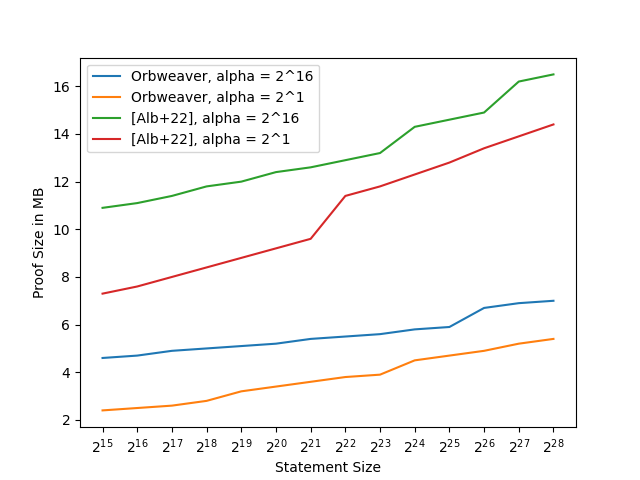
\includegraphics[width=\textwidth]{orbweaver/proofsizes}
        \end{center}
        \caption{Comparison of combined commitment and proof size for an unoptimized version of \sys and~\cite{C:ACLMT22} with $\ringdegree \geq 2^9$. We have purposely left errors in the code when producing the data in this figure for better comparison with~\cite{C:ACLMT22} (see details at the start of~\cref{sec:evaluation}).}
        \label{fig:proof-sizes}
\end{figure}


%%%%%%%%%%%%%%%%%%%%%%%%%%%%%%%%%%%%%%%%%%%%%%%%%%%%%%%%%%%%%%%%%%%%%%%%%%%%%%%%
%%%%%%%%%%%%%%%%%%%%%%%%%%%%%%%%%%%%%%%%%%%%%%%%%%%%%%%%%%%%%%%%%%%%%%%%%%%%%%%%
\subsection*{Acknowledgments}
\label{sec:acknowledgments}

We would like to thank Martin Albrecht and Russell W.F. Lai for answering questions about~\cite{C:ACLMT22}. We would also like to thank Nicholas Genise for answering our questions about lattice trapdoors.